\documentclass{swfcthesis}

\usepackage{xpinyin}
\usepackage{wrapfig}

\hypersetup{xetex,breaklinks=true,
  pdfinfo={
    Title={怎样用\LaTeX{}排版毕业论文},
    Author={王晓林},
    Keywords={latex, tutorial, 西南林业大学, 本科毕业论文模板, 教程, swfu},
  },
}

\setCJKfamilyfont{hei}{Adobe Heiti Std}
\setCJKfamilyfont{song}{Adobe Song Std}
\setCJKfamilyfont{kai}{Adobe Kaiti Std} % e.g. \CJKfamily{kai}
\newCJKfontfamily\cjkquotefont{Adobe Kaiti Std}

\addbibresource{tutorial.bib}

\newcommand{\Ca}{\LKeyCtrlX{a}}
\newcommand{\Cb}{\LKeyCtrlX{b}}
\newcommand{\Cc}{\LKeyCtrlX{c}}
\newcommand{\Cd}{\LKeyCtrlX{d}}
\newcommand{\Ce}{\LKeyCtrlX{e}}
\newcommand{\Cf}{\LKeyCtrlX{f}}
\newcommand{\Cg}{\LKeyCtrlX{g}}
\newcommand{\Ch}{\LKeyCtrlX{h}}
\newcommand{\Ci}{\LKeyCtrlX{i}}
\newcommand{\Cj}{\LKeyCtrlX{j}}
\newcommand{\Ck}{\LKeyCtrlX{k}}
\newcommand{\Cl}{\LKeyCtrlX{l}}
\newcommand{\Cm}{\LKeyCtrlX{m}}
\newcommand{\Cn}{\LKeyCtrlX{n}}
\newcommand{\Cp}{\LKeyCtrlX{p}}
\newcommand{\Cs}{\LKeyCtrlX{s}}
\newcommand{\Cv}{\LKeyCtrlX{v}}
\newcommand{\Cx}{\LKeyCtrlX{x}}
\newcommand{\Cy}{\LKeyCtrlX{y}}
\newcommand{\Cslash}{\LKeyCtrl{}+\biolinumKeyGlyph{slash}}
\newcommand{\Se}{\LKeyWin{}+\LKey{e}}
\newcommand{\Md}{\LKeyAltX{d}}
\newcommand{\Mv}{\LKeyAltX{v}}
\newcommand{\Mx}{\LKeyAltX{x}}
\newcommand{\MEnter}{\LKeyAlt{}+\LKeyEnter{}}
\newcommand{\Tab}{\LKeyTab{}}
\newcommand{\Enter}{\LKeyEnter{}}
\newcommand{\Caps}{\LKeyCapsLock{}}
\newcommand{\Ctrl}{\LKeyCtrl{}}

\begin{document}

\Title{怎样用\LaTeX{}排版毕业论文}% 论文标题
\Author{王晓林} % 作者姓名 
\Advisor{
\includegraphics[width=3em]{google-logo}} % 指导教师姓名
\AdvisorTitle{Titleless} % 指导教师职称

\AdvisorInfo{% 指导教师简介(约百余字)
  \noindent{}\texttt{{\large \$ dict google}}
  \begin{singlespace}
  \noindent{}\texttt{From The Free On-line Dictionary of Computing (05 May 2016) [foldoc]:}

  \begin{quote}{\ttfamily
      \hspace{-2em}Google
    
      <web> The \{web\} \{search engine\} that indexes the greatest number of web pages - over
      two billion by December 2001 and provides a free service that searches this index in
      less than a second.
  
      The site's name is apparently derived from "\{googol\}", but note the difference in
      spelling.
  
      The "Google" spelling is also used in "The Hitchhikers Guide to the Galaxy" by Douglas
      Adams, in which one of Deep Thought's designers asks, "And are you not," said Fook,
      leaning anxiously foward, "a greater analyst than the Googleplex Star Thinker in the
      Seventh Galaxy of Light and Ingenuity which can calculate the trajectory of every
      single dust particle throughout a five-week Dangrabad Beta sand blizzard?"
      
      \{(http://google.com/)\}.
      
      (2001-12-28) }
  \end{quote}
  \end{singlespace}
  % \begin{wrapfigure}{r}{.4\textwidth}
  %   \centering
  %   
\includegraphics[width=.39\textwidth]{albus}
  %   \caption*{By Source, Fair use, \url{https://en.wikipedia.org/w/index.php?curid=12991223}}
  % \end{wrapfigure}
  % Professor Albus Percival Wulfric Brian Dumbledore is a fictional character in
  % J. K. Rowling's Harry Potter series. For most of the series, he is the headmaster of the
  % wizarding school Hogwarts. As part of his backstory, it is revealed that he is the
  % founder and leader of the Order of the Phoenix, an organisation dedicated to fighting
  % Lord Voldemort.  Dumbledore is portrayed by Richard Harris in the film adaptations of
  % Harry Potter and the Philosopher's Stone and Harry Potter and the Chamber of
  % Secrets. After Harris' death, Michael Gambon portrayed Dumbledore for all of the
  % remaining films.  Rowling stated she chose the name Dumbledore, which is an Early Modern
  % English word for "bumblebee", because of Dumbledore's love of music: she imagined him
  % walking around "humming to himself a lot".\cite{wiki:albus}

  
  % 独孤求败,外号剑魔,是金庸小说中唯一被提及“真正无敌于天下”的高手,并当称为金庸
  % 小说世界中至高无上第一人。于小说中从未出场过,其事迹在极少数武林人士之间的口耳相传。其名
  % 字曾于金庸的三部小说中出现,分别为《神雕侠侣》、《笑傲江湖》以及《鹿鼎记
  % 》。\cite{wiki:duguqiubai}
  % \begin{itemize}
  % \item 《神雕侠侣》中,主角杨过习得独孤求败使用重剑以及其修练内力的法门后,继以晋身当代绝
  %   顶高手之列。
  % \item 《笑傲江湖》中,主角令狐冲原来武功平平,因缘际会学得独孤九剑以后,一跃为当代剑术高
  %   手。
  % \item 《鹿鼎记》一书中,实际上只有一句提及独孤求败,就是澄观和尚想及“无招胜有招”的前人例
  %   子时念起。
  % \end{itemize}
} 

\Year{二〇一六} 
\Month{六}
\Univ{西南林业大学}
\School{计算机与信息科学学院}
\Subject{计算机科学与技术专业}
\Docname{本科毕业(设计)论文}

\Abstract{% 论文摘要
  \LaTeX{}\footnote{\url{https://en.wikipedia.org/wiki/LaTeX}}是一种基
  于\TeX{}\footnote{\url{https://en.wikipedia.org/wiki/TeX}}的排版系统,由美国电脑学家莱斯
  利·兰伯特在20世纪80年代初期开发,利用这种格式,即使用户没有排版和程序设计的知识也可以充分
  发挥由TEX所提供的强大功能,能在几天,甚至几小时内生成很多具有书籍质量的印刷品。对于生成复
  杂表格和数学公式,这一点表现得尤为突出。因此它非常适用于生成高印刷质量的科技和数学类文档。
  这个系统同样适用于生成从简单的信件到完整书籍的所有其他种类的文档。\cite{wiki:latexcn}

  本文对如何利用\LaTeX{}来撰写西南林业大学本科毕业论文做一个简要的介绍。读者也可以将本文作
  为毕业论文模板来使用\footnote{本文所使用的毕业论文模板(\texttt{cls}文件),以及本文
    的\texttt{tex}源文件及相关文件都可以在下面的网址找
    到:\url{http://cs2.swfu.edu.cn/~wx672/swfcthesis/}}。}

\Keywords{\LaTeX{}, 西南林业大学, 本科毕业论文模板, 教程}% 关键词

\Acknowledgments{% 鸣谢 (感谢人民感谢党,约百字)
  感谢美国计算机教授高德纳(Donald Ervin Knuth)编写的功能强大的排版软件\TeX{}。感谢美国计
  算机科学家莱斯利·兰波特(Leslie Lamport)教授为\TeX{}开发的简单易用的\LaTeX{}宏包。感谢本
  文作者能有如此多的闲功夫和好心情来饶有兴致地做这样一件不能当饭吃的事情。}


\enTitle{How to write your dissertation with \LaTeX}% 英文标题
\enAuthor{WANG Xiaolin} % 作者英文姓名
\enUniv{Southwest Forestry University} % 英文校名
\enSchool{School of Computer and Information Science} % 英文院系名称

\enAbstract{% 论文英文摘要
  \LaTeX{} is a document preparation system. When writing, the writer uses plain text as
  opposed to formatted text as users of word processors like Microsoft Word. The writer
  uses markup tagging conventions to define the general structure of a document (such as
  article, book, and letter), to stylise text throughout a document (such as bold and
  italic), and to add citations and cross-references. A \TeX{} distribution such as
  \TeX{}Live or Mik\TeX{} is used to produce an output file (such as PDF or DVI) suitable
  for printing or digital distribution. Within the typesetting system, its name is
  stylised as \LaTeX{}.\cite{wiki:latex}

  This short tutorial shows you how to write an undergraduate dissertation in \LaTeX{}. It
  can also serve as a perfect template for your dissertation\footnote{The class file used
    for this thesis, and the \texttt{tex} source of this file can be found at
    \url{http://cs2.swfu.edu.cn/~wx672/swfcthesis/}.}.}

\enKeywords{\LaTeX{}, \TeX{}, tutorial, dissertation template, SWFU} % 英文关键字

%%% 下面六行不要动!
\makepreliminarypages
\frontmatter
\tableofcontents
\listoffigures
\listoftables
\mainmatter
%%% 上面六行不要动!

\chapter{工欲善其事,必先利其器} % 第一章标题
\label{cha:pre-requisite}

用\LaTeX{}撰写毕业论文是一件赏心乐事,前提是你得会。网上关于\LaTeX{}的入门教程很多,下面这
几个小教程就很不错,花一两天时间去熟悉一下,
\begin{enumerate}
\item \LaTeX{} from Wikibooks\footnote{\url{https://en.wikibooks.org/wiki/LaTeX}}
\item The very short guide to typesetting with
  \LaTeX{}\footnote{\url{http://tug.ctan.org/info/latex-veryshortguide/veryshortguide.pdf}}
\item The not so Short Introduction to
  \LaTeX{}\footnote{\url{https://www.ctan.org/tex-archive/info/lshort/english/?lang=en}}
\end{enumerate}
在有了对\LaTeX{}的基础认识之后,再接着往下看。

\section{工作环境}
\label{sec:env}

工作环境当然要清静、优雅。一杯热咖啡,配上轻音乐……除此之外,你还需要一台电脑,最好是像我用的电脑,
\begin{description}
\item[硬件:]不用太高级,但内存最好大一些,不少于4G为宜,因为在我看,CPU已经足够快了,电脑
  的运行速度更多的是取决于内存是否充足;
\item[操作系统:]Debian
  GNU/Linux\footnote{\url{https://en.wikipedia.org/wiki/Debian}}的Sid版。为什么不用MS
  Windows\footnote{\url{https://en.wikipedia.org/wiki/Microsoft_Windows}}? 因为~... 当然不是
  它不好,而是我缺乏足够的耐心。我的Debian Sid从来不考验我的耐心;
\item[桌面环境:]不需要。有个window manager就足够了。Sawfish window
  manager\footnote{\url{https://en.wikipedia.org/wiki/Sawfish_(window_manager)}},界面足够
  的简单,功能足够的丰富,配置足够的容易。而且它
  是Emacs\footnote{\url{https://en.wikipedia.org/wiki/Emacs}}的近亲,也
  是Lisp\footnote{\url{https://en.wikipedia.org/wiki/Lisp_(programming_language)}}的产物,
  这也许是我偏爱Sawfish的一个重要原因吧。

  如果你有个大屏幕,那么可以试
  试i3\footnote{\url{https://en.wikipedia.org/wiki/I3_(window_manager)}},一个很不错
  的tiling window
  manager\footnote{\url{https://en.wikipedia.org/wiki/Tiling_window_manager}}(平铺式窗口管
  理器)。它自动让所有的窗口互不重叠地铺满整个屏幕,非常适合大屏幕操作。对于我13吋的小屏
  幕,还是Sawfish更友好些,因为它能方便地让我全屏操作。

  除了窗口管理器,显然你还需要几个“窗口”。下面这三个恐怕是必须有的,
  \begin{itemize}
  \item Web浏览器,我用google-chrome;
  \item PDF阅读工具,我用zathura;
  \item 终端,我用xterm;
  \end{itemize}
\item[\LaTeX{}套件:]TeXLive\footnote{\url{https://en.wikipedia.org/wiki/TeX_Live}},它完备
  而庞大,我们只需要其中很少的一些软件包就够了;
\item[中文字体:]从你的Windows系统里拷贝过来就行了。相信我,这其实是你人生中唯一需要Windows的时
  候;
\item[编辑器:]Emacs + AUC\TeX{}\footnote{\url{https://en.wikipedia.org/wiki/AUCTeX}} +
  Yasnippet\footnote{\url{https://www.emacswiki.org/emacs/Yasnippet}};
  \begin{itemize}
  \item Emacs,世界上最强大的编辑器。\cite{emacs}作为计科专业的学生,如果你不熟悉它的使用,怎么好意思
    写毕业论文呢?
  \item AUC\TeX{}是一个历史悠久而强大的Emacs插件,它为我们编辑\LaTeX{}文件提供了丰富的快捷键操作;\cite{auctex}
  \item Yasnippet也是Emacs插件,它的功用就是为\Tab{}键施加魔法。\cite{yasnippet}有了它,期待奇迹出现的
    时候,你只要左手小指在\Tab{}键上轻轻一按……当然,你得先学会写魔咒(snippets)才
    行\,\Frowny{}。\label{p:yasnippet}
  \end{itemize}
  简而言之,有了上面两个插件,Emacs就成了一个强大的\LaTeX{}排版IDE\footnote{集成开发环境(Integrated
    Development Environment)。}。有了它,写起论文来,就像领导说套话一样顺滑流畅。
\end{description}

附录[\ref{app:pkg}]中列出了我的Debian系统上安装的与写论文相关的所有软件包,当然,清单里的
东西并非都是必需。其实,除了中文字体之外,其它的一切,你都可以根据自己的偏好来选择。如果你
打算用英文写论文的话,那么连中文字体都可以省略了。不管怎么说,上面提到的都是我个人的偏好,
本教程也将以此为基础,逐步展开。

至于如何安装、配置好这样一个工作环境……如果你是本校的学生,那么当然可以直截找我帮忙。如果你
不是本校的学生,那么……我曾经写过一个比较潦草
的\href{http://cs2.swfu.edu.cn/~wx672/lecture_notes/linux/install.html}{《Debian安装指
  导》}\cite{install},虽然有点旧了,但应该还是能对你有点帮助的。


\chapter{快速上手}

\LaTeX{}很强大,但对于初学者来说,你不必关心它有多强大,因为最为常用的命令和环境不过就是那么几
个。而且你也不必手工输入这些命令,只要你用Emacs+AUC\TeX{},几个简单的快捷键就足以满足你的基本
需求了。对于格式复杂的需求,通常你只要套用模版就可以解决问题了。所以,大家只要把Emacs用熟,
一切迎刃而解。

\section{用LaTeX写文章就是在编程}
\label{sec:hello}

\subsection{\texttt{hello.c}}
\label{sec:hello.c}

我们先回忆一下用Emacs写一个\texttt{hello.c}的键盘操作过程:
\begin{enumerate}
\item \Se{},如果你的系统配置和我的一样,那么只要按下\Se{}键,Emacs窗口就
  出现在你面前了,而且(感谢Sawfish)是全屏的;
\item \Cx \Cf{},开始编辑一个新文件。这时,在Emacs窗口的最下面(也就是 mini buffer 里)写
  上你要编辑的文件的名字,也就是\texttt{hello.c},然后按\Enter{}(回车键),或者\Cj{},其
  实,后面你会发现,\Cj{}带自动缩进,比按\Enter{}更方便;
\item 现在可以向你打开的空文件里写东西了;
  \begin{minted}[fontsize=\small,baselinestretch=1,
    linenos=true,numbersep=3pt,
    frame=leftline,framesep=10pt,rulecolor=\color{lightgray},
    xleftmargin=2cm,%,xrightmargin=4cm,
    gobble=2,
    ]{c}
    #include <stdio.h>
    int main()
    {
      printf ("Hello, world!\n");
      return 0;
    }
  \end{minted}
\item 存盘:\Cx \Cs{};
\item 编译:\texttt{gcc hello.c};
\item 运行:\texttt{./a.out};
\end{enumerate}

\subsection{\texttt{hello.tex}}
\label{sec:hello.tex}

现在,我们再看看用\LaTeX{}写一个\texttt{hello.tex}文件的过程:
\begin{enumerate}
\item \Se{},打开Emacs;
\item \Cx{} \Cf{},\texttt{hello.tex},开始编辑;
\item 写入文件内容;
  \begin{minted}[fontsize=\small,baselinestretch=1,
    linenos=true,numbersep=3pt,
    frame=leftline,framesep=10pt,rulecolor=\color{lightgray},
    xleftmargin=2cm,%xrightmargin=4cm,
    gobble=2
    ]{latex}
    \documentclass{article}
    \begin{document}
      Hello, world!
    \end{document}
  \end{minted}
\item 存盘:\Cx \Cs{};
\item 编译:\texttt{xelatex hello.tex};
\item 看结果:\texttt{xpdf hello.pdf}。
\end{enumerate}

怎么样? \texttt{hello.c}和\texttt{hello.tex}的编辑过程没什么分别吧。只要把Emacs用熟练,触
类旁通,不管写什么程序,都是这么个过程。你
\begin{itemize}
\item 不必学习VC去写C/C++;
\item 不必学习eclipse去写Java;
\item 不必学习MS-Word去写报告、幻灯片;
\item 不必学习……
\end{itemize}
一句话,“Everything Emacs”,你可以省下大量不必要的学习时间。人生苦短,何必让你的生活
被 VC/eclipse/MS-Word 搞得头昏脑胀呢? 简单而强大,本就是计科专业学生和非专业学生应有的不
同。

如果你对Emacs操作还很陌生,那么现在就打开Emacs,\Ch{} \LKey{t},重温一下那些基本操
作吧。

\subsection{什么是 \Cx \Cf?}

使用Emacs是可以(而且应该)完全抛开鼠标的。对于初次上手的人,抛开鼠标就像病人抛开拐杖一
样痛苦。但只有不依赖拐杖的人才是健康的,不是吗?

现在,你终于有了走向健康生活的冲动,那么我们开始吧。简短截说,
\begin{enumerate}
\item 先把你的双手在标准键盘上放好。然后,
\item 左手小指稍向左移,按在\Caps{}(CapsLock)键上\footnote{如果你的系统配置和我一
    样,那么\Caps{}就是\Ctrl{}键。},按住别放开,
\item 左手无名指稍向下移,在\LKey{x}键上轻按一下就放开,这就是\Cx{}。 
\item 小指按在\Caps{}上别放开,左手食指在\LKey{f}键上轻按一下就放开,这就是\Cf{}。
\item 现在左手小指可以放开了。
\end{enumerate}
这就是\Cx \Cf{},最常用的Emacs快捷键之一,作用是要求打开一个文
件\footnote{如果你要打开的文件不存在,那么Emacs会认为你要写一个新文件。},f代表file 。那么,
告诉我
\begin{itemize}
\item 什么是 \LKeyCtrlX{x} \LKeyCtrlX{s}?
\item 什么是 \LKeyCtrlX{x} \LKey{2}? 什么是\LKeyCtrlX{x} \LKey{3}? 什么是\LKeyCtrlX{x}
  \LKey{0}? 什么是\LKeyCtrlX{x} \LKey{1}? 什么是\LKeyCtrlX{x} \LKey{o}?
\item 什么是\LKeyCtrlX{x} \LKey{h}? 什么是\LKeyCtrlX{w}?
\item 什么是 \LKeyCtrlX{g}?
\item 什么是\LKeyCtrlX{j}? 什么是 \LKeyCtrlX{i}?
  % \item 什么是 \LKeyCtrlX{/}?
\item 什么是 \LKeyCtrlX{k}? 什么是 \LKeyCtrlX{y}?
\item 什么是\LKeyCtrlX{d}? 什么是 \LKeyAltX{d}?% (M 代表 Meta 键, 也就是 Alt 键)
\item 什么是 \LKeyCtrlX{a}? 什么是\LKeyCtrlX{e}? 什么是\LKeyCtrlX{f}? 什么是\LKeyCtrlX{b}?
  什么是\LKeyCtrlX{n}? 什么是\LKeyCtrlX{p}?
\end{itemize}
如果你还不熟悉上面这些快捷键,那么用起Emacs来,就会像西洋人用筷子一样不酷。(「嘿!把你的手从
鼠标上拿开!」)刚甩开拐杖,走向健康生活的人,总会不自觉地去扶点什么,这很正常。但你一定要坚
持锻炼,不要让这种「正常」持续得太久。今后的生活能否轻松愉快,主要就取决于你的「健康」程度。
如果有朝一日你真的抛开了鼠标,那么即使面对一个纯字符界面的终端,你也能写出漂亮的PDF格式的论
文。作为计科专业的学生,好歹该比网吧青年们酷一些嘛。

\section{生活可以更轻松}

AUC\TeX{}是Emacs的一个功能模块,为\LaTeX{}编程提供了巨大的便利。有了它,你的\LaTeX{}生活可以
像 \texttt{Hello, world!}一样简单。现在就跟着我,手把手地领略一下简单的乐趣吧。

一切当然是从\LKeyWin{}+\LKey{e},打开Emacs开始。然后,\LKeyCtrlX{x} \LKeyCtrlX{f},让我们开
始编辑一个新文件,就叫 \texttt{simple.tex}吧。

在Emacs窗口的最下方,也就是 mini buffer 里,这时应该会有提示,让你输入文件名。输
入\texttt{simple.tex}, 然后按 \LKeyCtrlX{j}。如果这时 mini buffer 里有如下提示:
\begin{itemize}
\item[] \texttt{Master file: (default this file) ...}
\end{itemize}
直接按 \Cj{} 就可以了。知道了吧, \Cj{} 就是我们的\Enter{}(回车)键。如果你的手正放在「标准
键盘」上,那么,左手小指向左一偏,按到的正是\Ctrl{}键(\Caps{}{\scriptsize (CapsLock)}被我
们改造成\Ctrl{}了)。右手食指下不正是\LKey{j}键吗?怎么样,比\Enter{}更方便吧。

现在,可以向 \texttt{simple.tex}文件里写东西了,\Cc \Ce{},e代表environment。“环境”到底是什么
呢?意会吧,用用就明白了。在 mini buffer 里会有提示,
\begin{itemize}
\item[] \texttt{Environment type: (default document)}
\end{itemize}
这是在问你是不是要写一篇document(文章)啊?你当然该用\Cj{}来告诉它「是」。这时,mini buffer 又会提示,
\begin{itemize}
\item[] \texttt{Document class: (default article)}
\end{itemize}
这是在问你是不是要写一篇 article 类型的文章啊?除了 article,通常还有 book, report, letter
可供选择。我们现在碰巧就是要写个短小的 article,所以,按\Cj{}确认就好。这时, mini buffer 继续提示,
\begin{itemize}
\item[] \texttt{Options:}
\end{itemize}
这是在问你是否有什么特殊选项啊?用\Cj{}来告诉它说「不需要」。现在,你的 \texttt{simple.tex}
文件里应该有如下几行东西了:
\begin{minted}[fontsize=\small,baselinestretch=1,
  linenos=true,numbersep=3pt,
  frame=leftline,framesep=10pt,rulecolor=\color{lightgray},
  xleftmargin=2cm,%xrightmargin=4cm,
  gobble=2
  ]{latex}
  \documentclass{article}  % documentclass可以是
                           % article, book, report, letter...
  \begin{document}         % 文章的开始
  | 
  \end{document}           % 文章的结束
\end{minted}

这时,光标停在 \verb|\begin{document}|与 \verb|\end{document}|之间,等待你的输入。百分号
(\verb|%|)后面显然都是注释。

在第\ref{sec:hello}节里,你已经会写 \texttt{Hello, world!}了。现在,我们要写点像模像样的东西。
偷懒起见,我直接套{\tiny (\pinyin{chao1})}用{\tiny (\pinyin{xi2})} Andrew
Roberts 写的
\texttt{simple.tex}\footnote{\url{http://en.wikibooks.org/wiki/LaTeX/simple.tex}}\cite{simple}
。我们把注意力集中在用Emacs写文章的过程上。

\subsection{Top matter}

先确保你的光标在 \verb|\begin{document}| 和 \verb|\end{document}| 之间,也就是文章的
第4行。然后按\Cc \Cm{},这时 mini buffer 里会有如下提示:
\begin{itemize}
\item[] \verb|Macro (default ref): \|
\end{itemize}
这是系统在等待你输入一个 \texttt{Macro},说白了就是“命令”。输入:\texttt{title},\Cj{},这时
你的文章会变成下面这样:
\begin{minted}[fontsize=\small,baselinestretch=1,
  linenos=true,numbersep=3pt,
  frame=leftline,framesep=10pt,rulecolor=\color{lightgray},
  xleftmargin=2cm,%xrightmargin=4cm,
  gobble=2
  ]{latex}
  \documentclass{article}  % documentclass可以是
                           % article, book, report, letter...
  \begin{document}         % 文章的开始
  \title{|} 
  \end{document}           % 文章的结束
\end{minted}
这时,光标停在 \verb|\title{}| 的花括号里。不用说你也知道,该输入文章的标题了。那么就给它
一个标题:
\begin{minted}[fontsize=\small,baselinestretch=1,
  linenos=true,numbersep=3pt,
  frame=leftline,framesep=10pt,rulecolor=\color{lightgray},
  xleftmargin=2cm,%xrightmargin=4cm,
  gobble=2
  ]{latex}
  \documentclass{article}  % documentclass可以是
                           % article, book, report, letter...
  \begin{document}         % 文章的开始
  \title{How to Structure a \LaTeX{} Document} 
  \end{document}           % 文章的结束
\end{minted}
发现了吗?凡是以反斜杠开头的都是命令(\texttt{Macro}), 比如 \verb|\LaTeX{}|,它的唯一作用
就是把 \texttt{LaTeX} 这五个字母输出成一副怪样子,\LaTeX{}。

好了,在 title 下新起一行。然后\Cm{}。你肯定知道 \Cm{}是干什么用的了吧,就是要输入一
个 Macro。也许你会好奇,想知道总共有多少 Macro? 那么现在可以按一下\Tab{}键。看到了吗?在弹
出的新窗口中,列出了近百个 Macro. 还好,我们并不需要记住这么多。最常用的也就三、五个而已。

mini buffer 里又会有提示:
\begin{itemize}
\item[] \verb|Macro (default title): \|
\end{itemize}
Emacs会把我们上次输入的Macro,也就是title,做为默认值提示出来。不用管它,输入:
\texttt{author} \Cj{}。然后在 \verb|\author{}| 的花括号里输入作者的名字。当然,也可以把自己
的通信地址、email写在里面。就像下面这样:

\begin{minted}[fontsize=\small,baselinestretch=1,
  linenos=true,numbersep=3pt,
  frame=leftline,framesep=10pt,rulecolor=\color{lightgray},
  xleftmargin=2cm,%xrightmargin=4cm,
  gobble=2
  ]{latex}
  \documentclass{article}  % documentclass可以是
                           % article, book, report, letter...
  \begin{document}         % 文章的开始
  \title{How to Structure a \LaTeX{} Document}
  \author{Andrew Roberts\\
    School of Computing,\\
    University of Leeds,\\
    Leeds,\\
    United Kingdom,\\
    LS2 1HE\\
    \emph{andyr@comp.leeds.ac.uk}}
  \end{document}           % 文章的结束
\end{minted}

注意,\verb|\\|代表“强制换行”。现在,新起一行,加上日期:
\begin{enumerate}
\item \Cc\Cm{} date \Cj
\item \Cc\Cm{} today \Cj
\end{enumerate}
其实,如果没有 \verb|\date{\today}| 这一句,系统会自动把今天的日期添加上的。而
且 \verb|\date{}|里面的日期你可以随意写,不一定非要是当天的日期。title, author, date 一般被
叫做文章的 top matter(开头那点事)。

再新起一行,写 \verb|\maketitle| \Cj{}。\verb|\maketitle| 自然是要排版top matter了。换句
话说,不要标题的话可以省略掉这个命令。现在文章变成了这样:

\begin{minted}[fontsize=\small,baselinestretch=1,
  linenos=true,numbersep=3pt,
  frame=leftline,framesep=10pt,rulecolor=\color{lightgray},
  xleftmargin=2cm,%xrightmargin=4cm,
  gobble=2
  ]{latex}
  \documentclass{article}  % documentclass可以是
                           % article, book, report, letter...
  \begin{document}         % 文章的开始
  \title{How to Structure a \LaTeX{} Document}
  \author{Andrew Roberts\\
    School of Computing,\\
    University of Leeds,\\
    Leeds,\\
    United Kingdom,\\
    LS2 1HE\\
    \emph{andyr@comp.leeds.ac.uk}}
  \date{\today}
  \maketitle
  \end{document}           % 文章的结束
\end{minted}

好奇的话,现在可以编译一下,看看PDF文件的效果:
\begin{enumerate}
\item 编译:\Cc\Cc\Cj
\item 查看:\Cc\Cv
\end{enumerate}
这时,一个PDF文件应该显示在屏幕上了。效果还满意吧?保持你的好奇心。在下面的操作中,你随时可
以编译一下看看效果。

\begin{center}
  \fbox{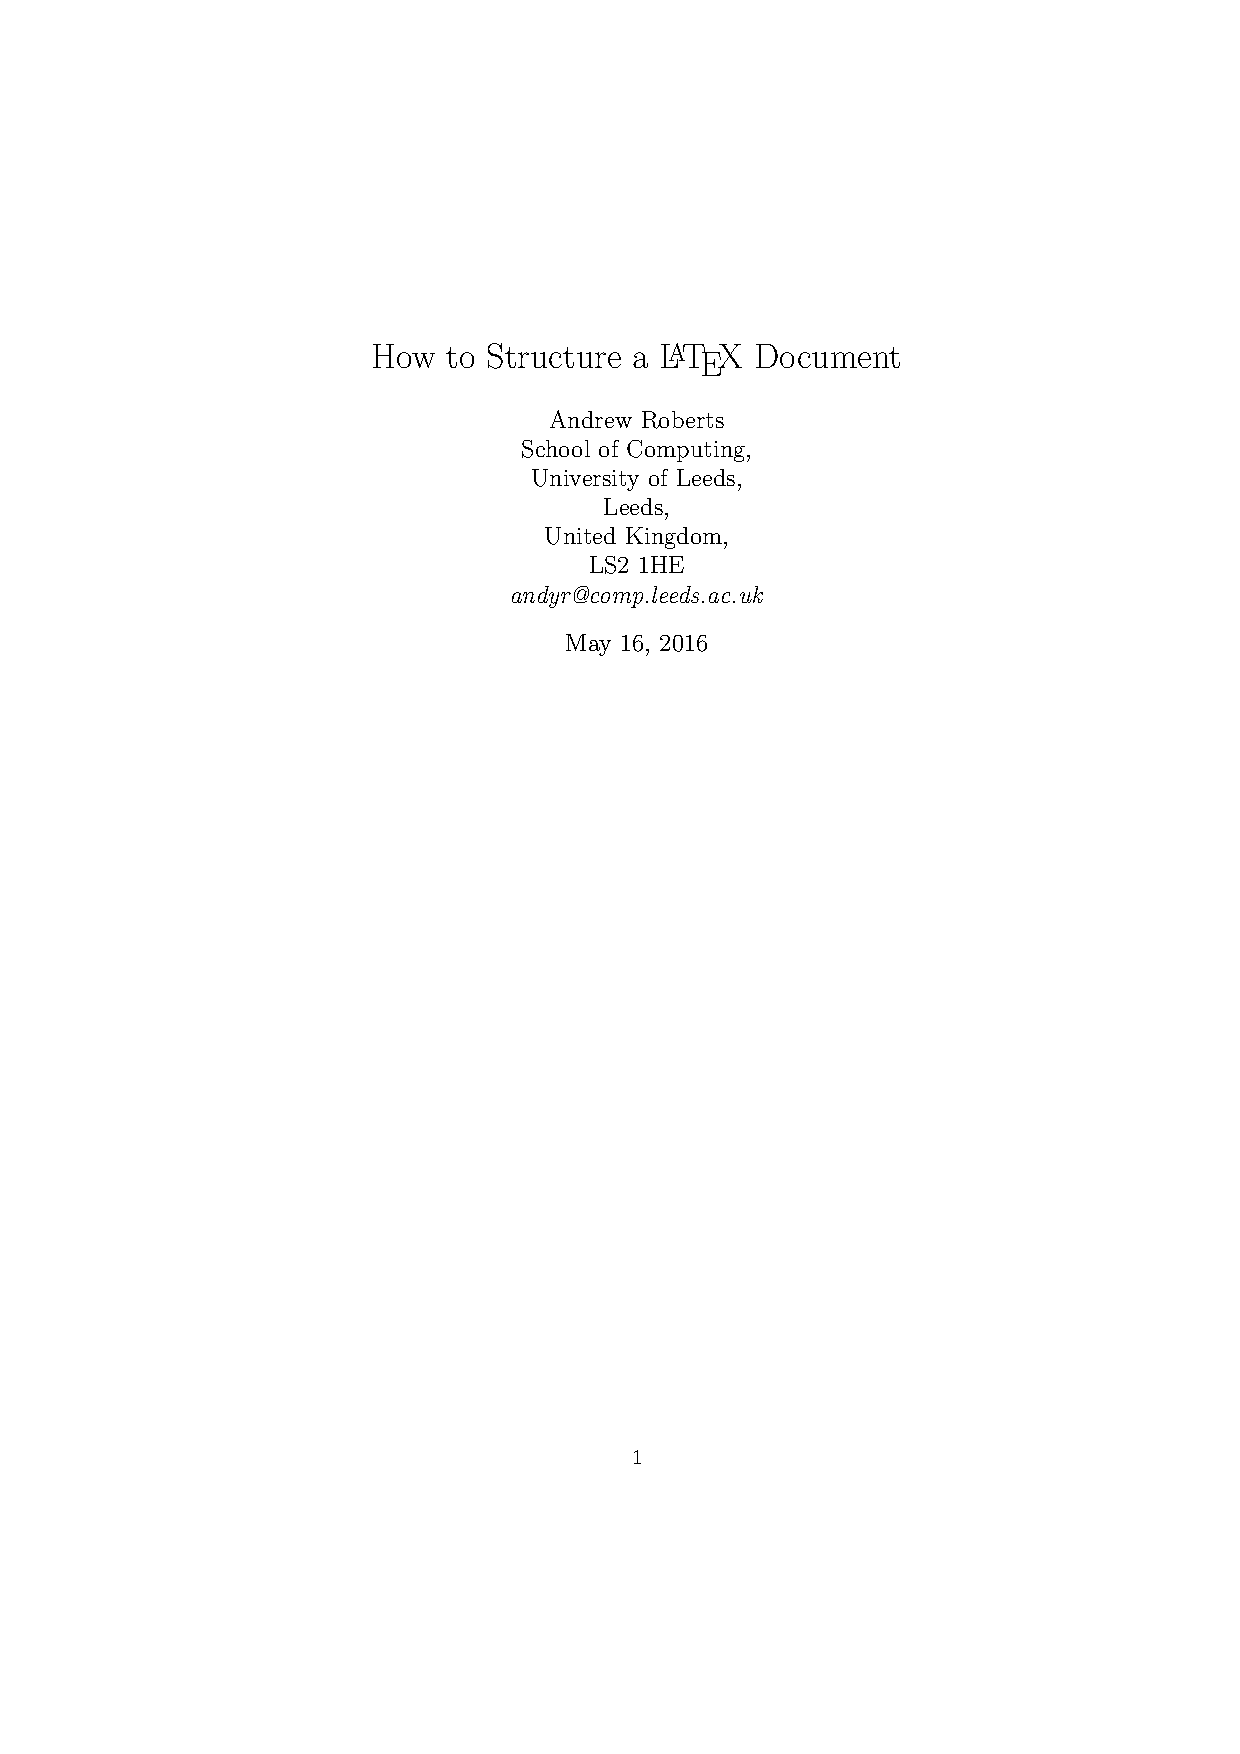
\includegraphics[width=.6\textwidth]{topmatter}}
\end{center}

\subsection{怎样写摘要}

好了,回到Emacs。现在你的光标应该停在 \verb|\maketitle| 的下面一行。我们开始写「摘要」部
分。\Cc\Ce{},开始一个新的“环境”\footnote{如果你好奇心强,想知道总共有哪些“环境”的话,现在
  可以按\Tab{}键。}。mini buffer 里提示:
\begin{itemize}
\item[] \texttt{Environment type: (default itemize)}
\end{itemize}
这是在问你要开始哪个环境啊?默认是开始 itemize 环境,因为它是最常用的环境。但我们现在要写的是“摘要”,告诉它:
abstract \Cj{}。abstract 就是“摘要”的意思。科技论文都是要有摘要的嘛。于是,你的文章变成了这样:

\begin{minted}[fontsize=\small,baselinestretch=1,
  linenos=true,numbersep=3pt,
  frame=leftline,framesep=10pt,rulecolor=\color{lightgray},
  xleftmargin=2cm,%xrightmargin=4cm,
  gobble=2
  ]{latex}
  % 此处略去十数行
 
  \maketitle
 
  \begin{abstract} 
    |
  \end{abstract}
  \end{document}           % 文章的结束
\end{minted}

光标停在 \verb|\begin{abstract}| 和 \verb|\end{abstract}| 之间(第6行)。好,现在往摘要部分里填点东西:

\begin{minted}[fontsize=\small,baselinestretch=1,
  linenos=true,numbersep=3pt,
  frame=leftline,framesep=10pt,rulecolor=\color{lightgray},
  xleftmargin=2cm,%xrightmargin=4cm,
  gobble=2
  ]{latex}
  % 此处略去十数行
 
  \maketitle
 
  \begin{abstract} 
    In this article, I shall discuss some of the fundamental
    topics in producing a structured document.  This document
    itself does not go into much depth, but is instead the
    output of an example of how to implement structure. Its
    \LaTeX{} source, when in used with my tutorial provides
    all the relevant information.
  \end{abstract}
  \end{document}           % 文章的结束
\end{minted}

看看效果:
\begin{center}
  \fbox{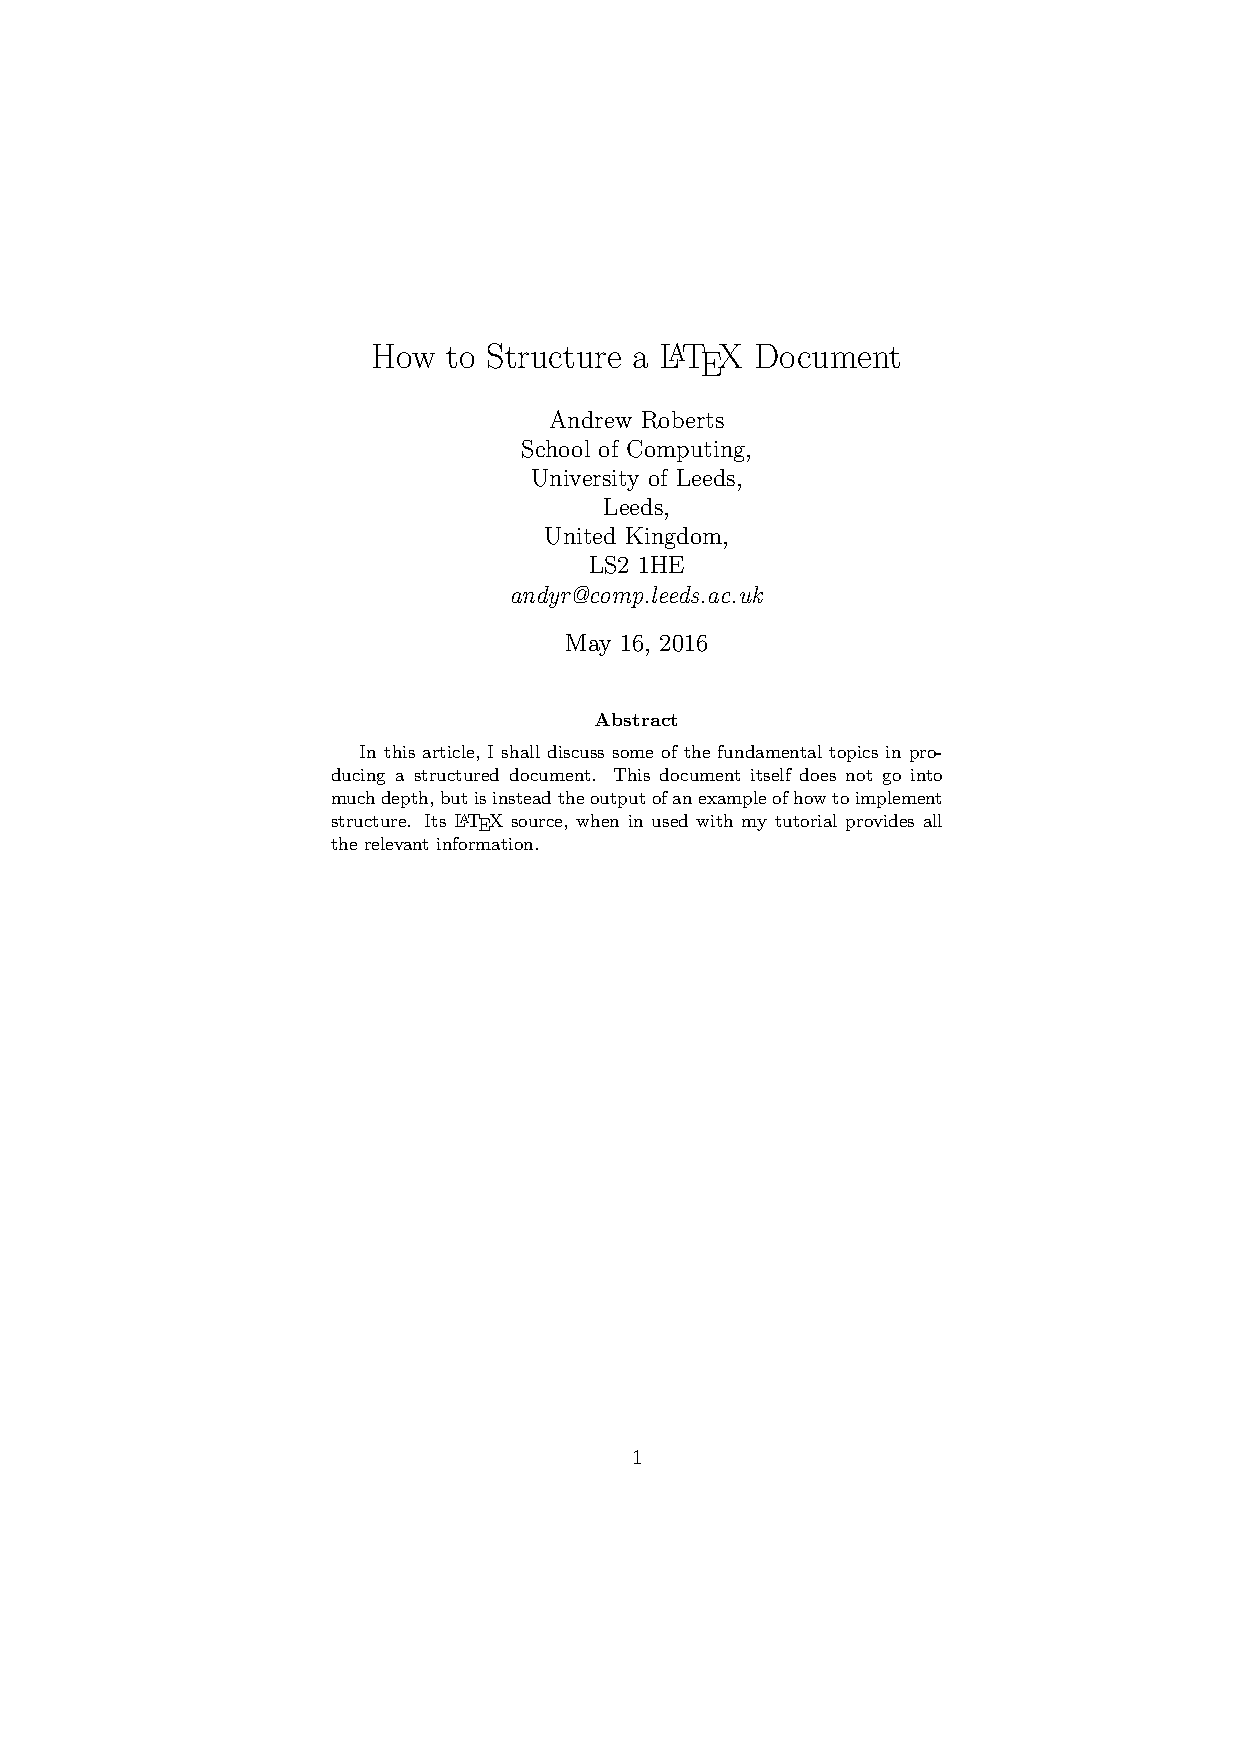
\includegraphics[width=.45\textwidth]{abstract}}
\end{center}

\subsection{怎样分章节}

现在,我们要接着上面的例子,写更多更长的东西了。偷懒起见,文章末尾的 \verb|\end{document}|
我也不再写出来了。

好,按\Cn{}把光标移到 \verb|\end{abstract}| 的下一行。然后,\Cc\Cs{},让我们开始文章的第一节。
s 代表 section, “节”的意思。mini buffer 提示:
\begin{itemize}
\item[] \texttt{Level: (default section) }
\end{itemize}
显然是在问你,要不要起一个新 section 啊?没错,我就是要起一个新的章节,于是直接\Cj{}。
mini buffer 又提示:
\begin{itemize}
\item[] \texttt{Title:}
\end{itemize}
也就是问你,章节标题是……?那就给它个标题吧,就叫“Introduction”。\Cj{}之后, mini buffer 继续提示:
\begin{itemize}
\item[] \texttt{Label: sec:introduction}
\end{itemize}
这是在问你,要不要给这个新章节打个标签,比如 \texttt{sec:introduction}, 以后也许要索引到它呢?
这个暂时无关紧要,\Cj{}就行了。于是,文中又有了下面的第5、6两行。

\begin{minted}[fontsize=\small,baselinestretch=1,
  linenos=true,numbersep=3pt,
  frame=leftline,framesep=10pt,rulecolor=\color{lightgray},
  xleftmargin=2cm,%xrightmargin=4cm,
  gobble=2
  ]{latex}
  % 此处略去十数行

  \end{abstract}

  \section{Introduction}
  \label{sec:introduction}
\end{minted}

给这一节添加内容:

\begin{minted}[fontsize=\small,baselinestretch=1,
  linenos=true,numbersep=3pt,
  frame=leftline,framesep=10pt,rulecolor=\color{lightgray},
  xleftmargin=2cm,%xrightmargin=4cm,
  gobble=2
  ]{latex}
  % 此处略去十数行

  \end{abstract}

  \section{Introduction}
  \label{sec:introduction}

  This small document is designed to illustrate how easy
  it is to create a well structured document within
  \LaTeX\cite{lamport94}.  You should quickly be able to
  see how the article looks very professional, despite the
  content being far from academic.  Titles, section headings,
  justified text, text formatting etc., is all there, and
  you would be surprised when you see just how little markup
  was required to get this output.
\end{minted}

注意到了吗?在这一节里有一个新命令 \verb|\cite{}|, 这是在引用一个参考文献。先不管它,后面再说。

如法炮制,再添加几个章节:

\begin{minted}[fontsize=\small,baselinestretch=1,
  linenos=true,numbersep=3pt,
  frame=leftline,framesep=10pt,rulecolor=\color{lightgray},
  xleftmargin=2cm,%xrightmargin=4cm,
  gobble=2
  ]{latex}
  % 此处略去十数行

  \end{abstract}

  \section{Introduction}
  \label{sec:introduction}

  This small document is designed to illustrate how easy
  it is to create a well structured document within
  \LaTeX\cite{lamport94}.  You should quickly be able to
  see how the article looks very professional, despite the
  content being far from academic.  Titles, section headings,
  justified text, text formatting etc., is all there, and
  you would be surprised when you see just how little markup
  was required to get this output.

  \section{Structure}
  \label{sec:structure}
  
  One of the great advantages of \LaTeX{} is that all it needs
  to know is the structure of a document, and then it will
  take care of the layout and presentation itself. So, here we
  shall begin looking at how exactly you tell \LaTeX{} what it
  needs to know about your document.
  
  \subsection{Top Matter}
  \label{sec:top-matter}
  
  The first thing you normally have is a title of the document,
  as well as information about the author and date of publication.
  In \LaTeX{} terms, this is all generally referred to as
  \emph{top matter}.

  |
\end{minted}

注意到 \verb|\emph{}| 了吗?它代表 emphasize ,“强调”。英文习惯用斜体字来表示强调的东西,那
么 \verb|\emph{hello, world}| 自然就是把 hello, world 排版成 \emph{hello, world} 了。

注意到 \verb|\subsection{}| 了吗?一会儿,我们还会看到 \verb|\subsubsection|。不用解释吧,
文章的章节次序是这样:

\begin{enumerate}
\item chapter
\item section
\item subsection
\item subsubsection
\item paragraph
\item subparagraph
\end{enumerate}
其中的chapter,只有在 book 和 report 中才能使用,而 article 只能用 section 以下的东西。

现在我们就来增加一个 subsubsection。不出所料的话,光标现在应该在第34行。那么
就\Cc\Cs{},mini buffer 提示:
\begin{itemize}
\item[] \texttt{Level: (default subsection)}
\end{itemize}
当然输入:subsubsection \Cj{}。mini buffer 提示:
\begin{itemize}
\item[] Title:
\end{itemize}
输入:Article Information \Cj。mini buffer 提示:
\begin{itemize}
\item[] \texttt{Label: sec:article-information}
\end{itemize}
似曾相识吧?敲\Cj{},于是,文章中又有了如下两行:

\begin{minted}[fontsize=\small,baselinestretch=1,
  linenos=true,numbersep=3pt,
  frame=leftline,framesep=10pt,rulecolor=\color{lightgray},
  xleftmargin=2cm,%xrightmargin=4cm,
  gobble=2
  ]{latex}
  \subsubsection{Article Information}
  \label{sec:article-information}
\end{minted}

也就是说,我们有了一个 subsubsection。

\subsection{什么是环境}

现在,我们来添加一个 environment。\Cc\Ce{},mini buffer 提示:
\begin{itemize}
\item[] \texttt{Environment type: (default abstract)}
\end{itemize}
我们当然不再需要 abstract 了,现在我们要的是 itemize ,也就是“不带序号的列表”。那么当然输
入:itemize \Cj{}。于是看到:

\begin{minted}[fontsize=\small,baselinestretch=1,
  linenos=true,numbersep=3pt,
  frame=leftline,framesep=10pt,rulecolor=\color{lightgray},
  xleftmargin=2cm,%xrightmargin=4cm,
  gobble=2
  ]{latex}
  \begin{itemize}
  \item |
  \end{itemize}
\end{minted}

光标停在 \verb|\item| 的后面。非常好,这正是我想要的。于是直接输入如下文字:
\begin{itemize}
\item[] \verb'\verb|\title{}| --- The title of the article.'
\end{itemize}
输入之后,\MEnter{},也就是,左手拇指按住\LKeyAlt{}键,同时右手小指去敲\Enter{}。你会看到
这样的效果:

\begin{minted}[fontsize=\small,baselinestretch=1,
  linenos=true,numbersep=3pt,
  frame=leftline,framesep=10pt,rulecolor=\color{lightgray},
  xleftmargin=2cm,%xrightmargin=4cm,
  gobble=2
  ]{latex}
  \begin{itemize}
  \item \verb|\title{}| --- The title of the article.
  \item 
  \end{itemize}
\end{minted}

也就是说,不仅换了行,而且自动有了 \verb|\item|等待你输入新的东西。

你一定注意到了 \verb'\verb||' 这个新命令。它的作用和bash命令行的单引号 (\texttt{'}) 是一样的。
还记得吧,在命令行,单引号里的东西是原样输出的。 \verb'\verb||' 里的东西也一样。 verb 是
verbatim 一词的缩写,就是“原样引用”的意思。好奇的话,可以编译一下,看看效果。

\begin{center}
  \fbox{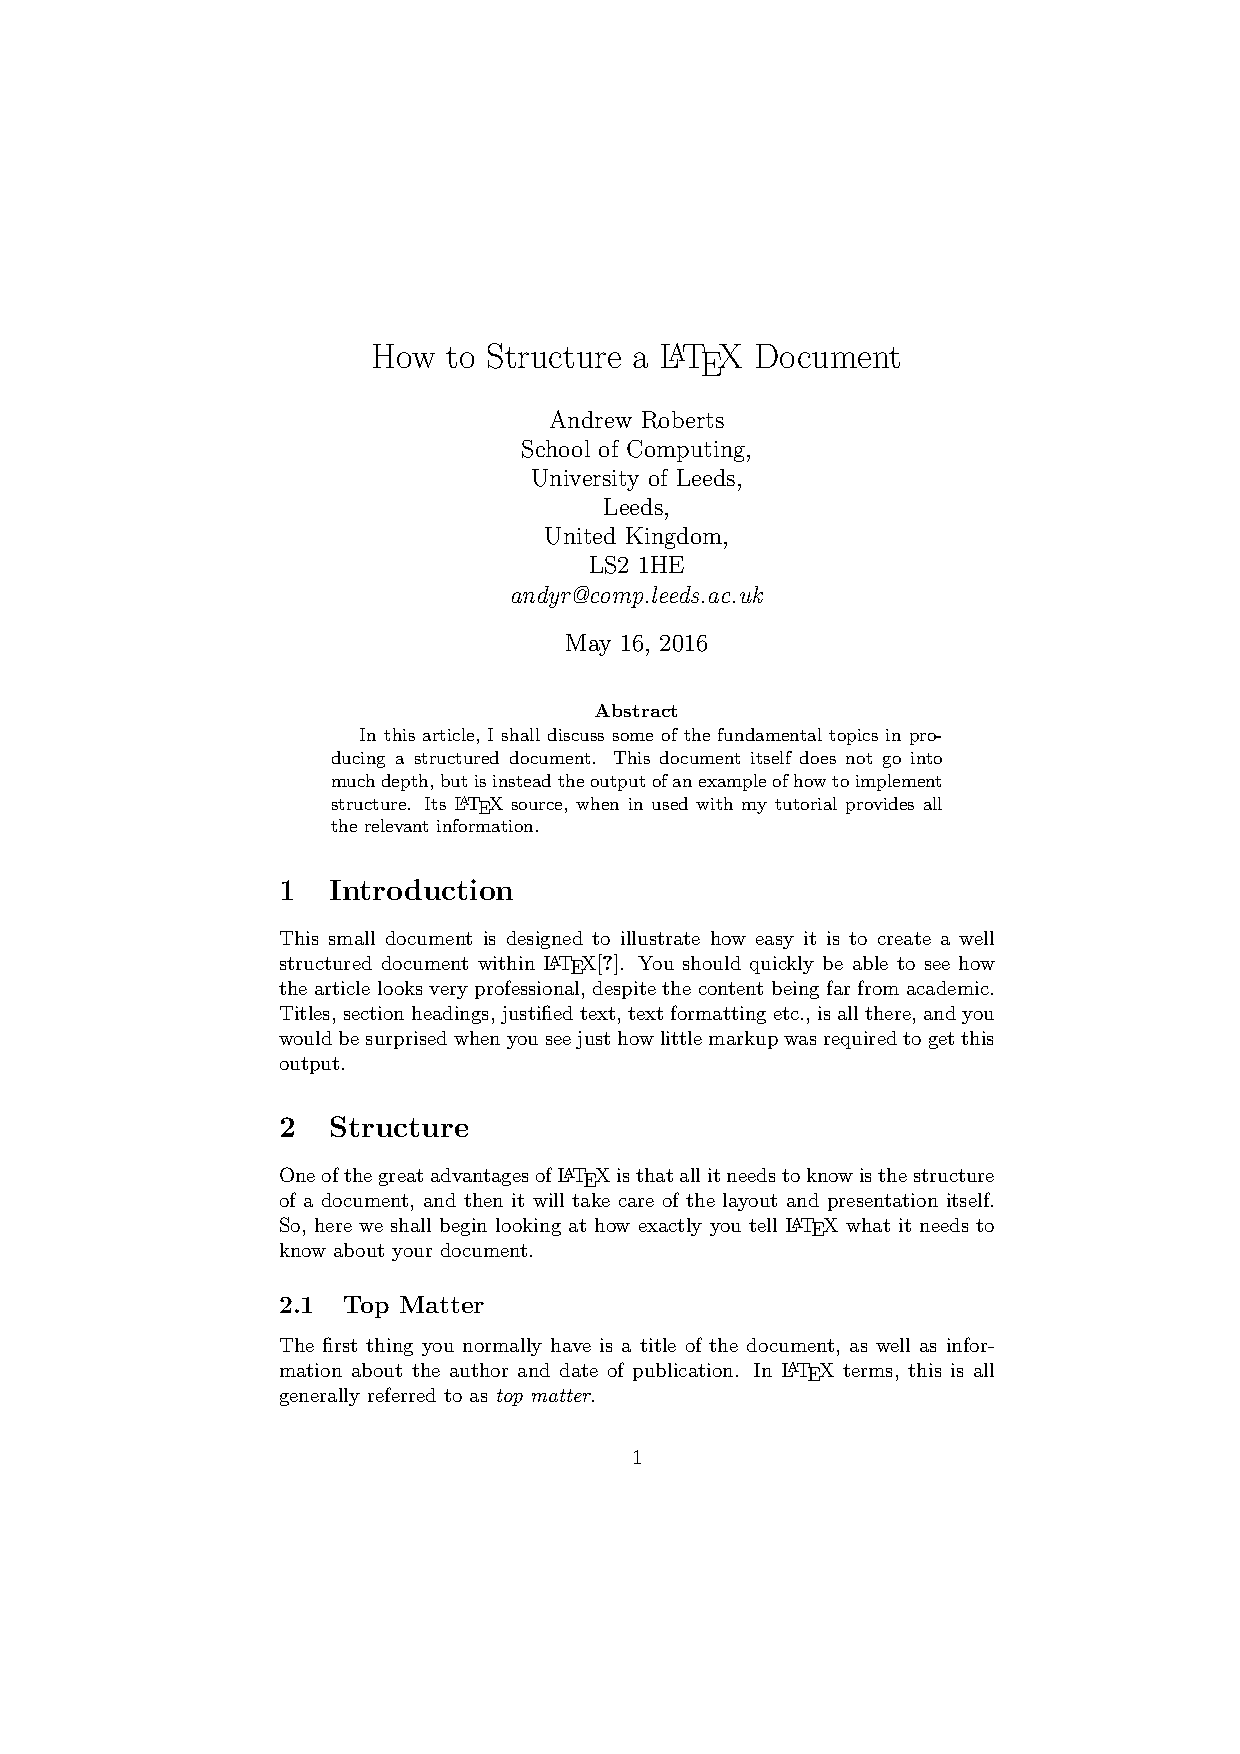
\includegraphics[width=.48\textwidth]{env1}}
  \fbox{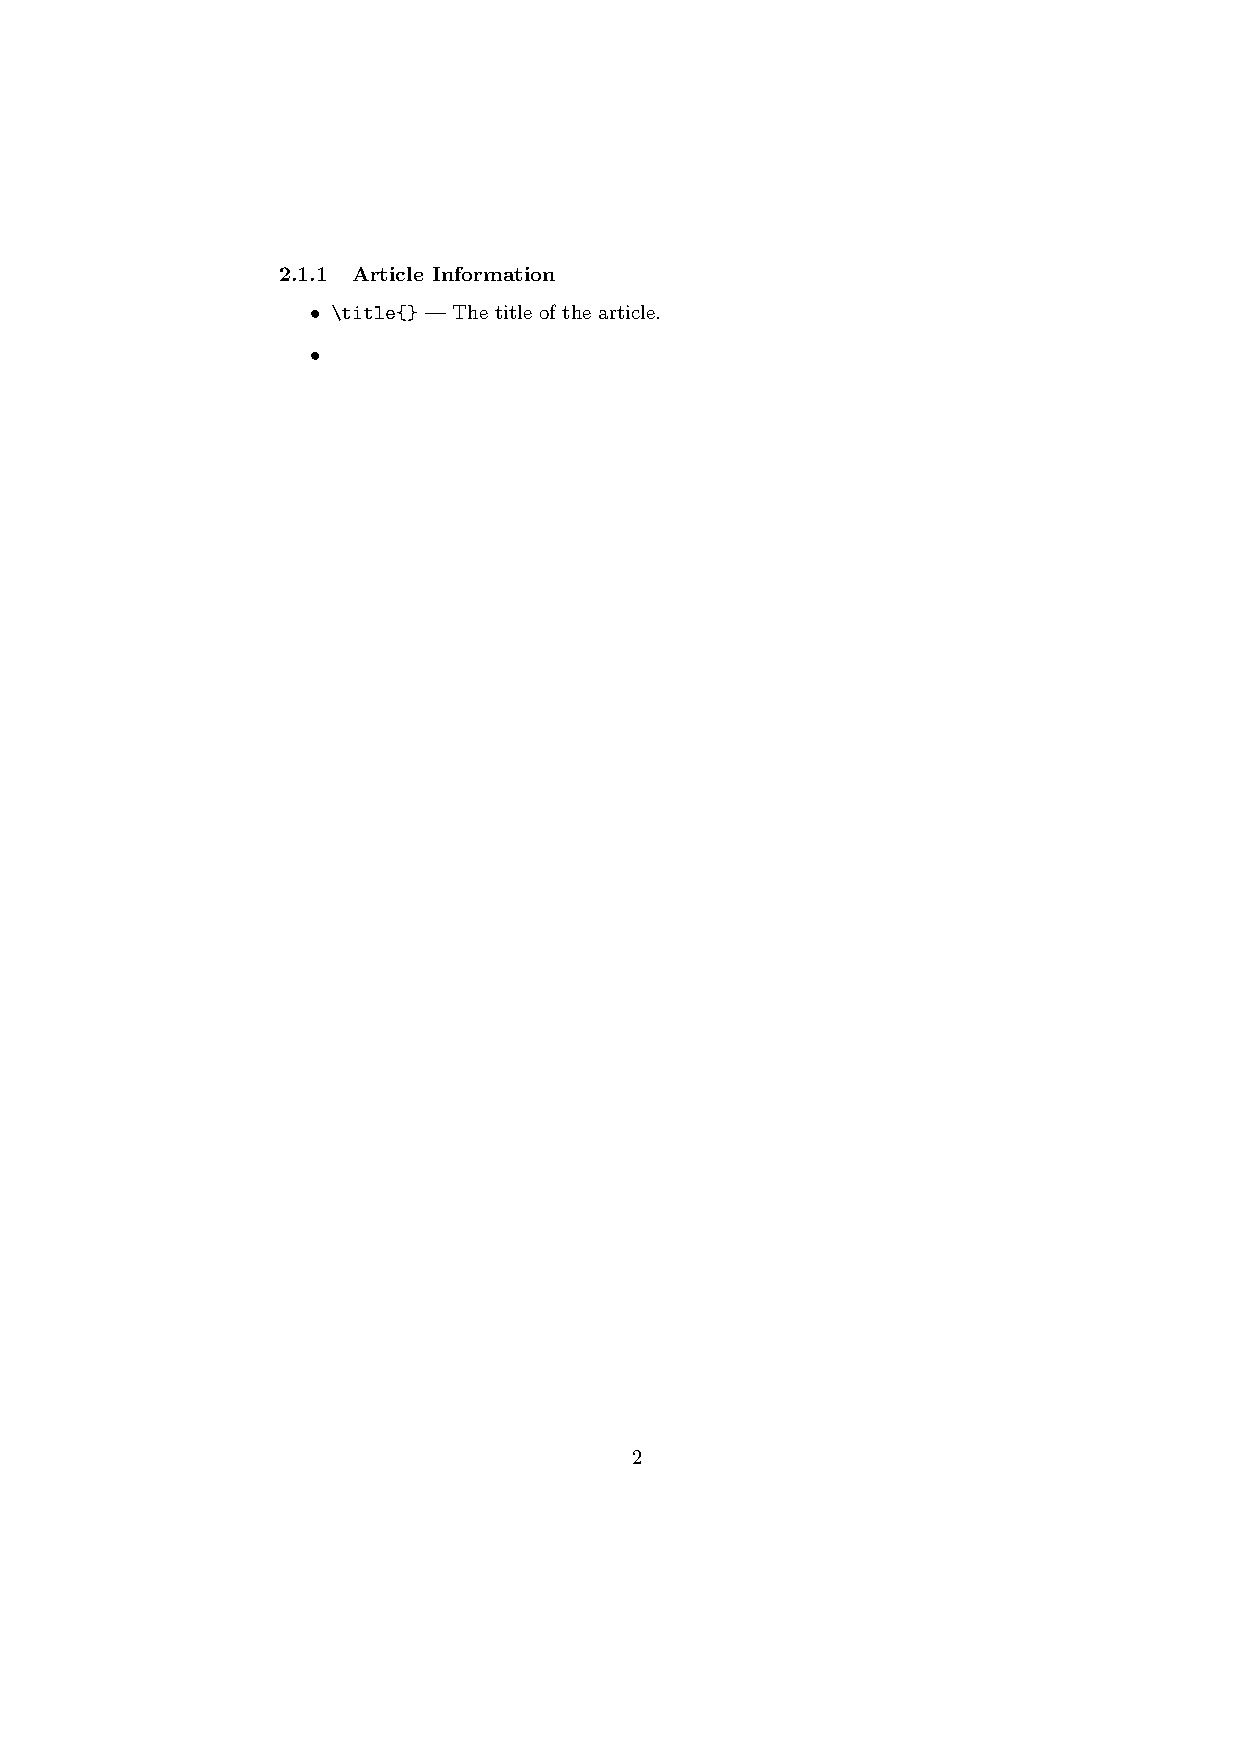
\includegraphics[width=.48\textwidth]{env2}}
\end{center}

好,继续输入:
\begin{itemize}
\item[] \verb'\verb|\date| --- The date. Use:'
\end{itemize}
得到:

\begin{minted}[fontsize=\small,baselinestretch=1,
  linenos=true,numbersep=3pt,
  frame=leftline,framesep=10pt,rulecolor=\color{lightgray},
  xleftmargin=2cm,%xrightmargin=4cm,
  gobble=2
  ]{latex}
  \begin{itemize}
  \item \verb|\title{}| --- The title of the article.
  \item \verb|\date| --- The date. Use: 
  \end{itemize}
\end{minted}

没什么好说的。现在我们要在 itemize 环境里面再套一个 itemize 。光标现在应该在第3行的最后。
敲:\Cc\Ce\Cj{},于是得到:

\begin{minted}[fontsize=\small,baselinestretch=1,
  linenos=true,numbersep=3pt,
  frame=leftline,framesep=10pt,rulecolor=\color{lightgray},
  xleftmargin=2cm,%xrightmargin=4cm,
  gobble=2
  ]{latex}
  \begin{itemize}
  \item \verb|\title{}| --- The title of the article.
  \item \verb|\date| --- The date. Use:
    \begin{itemize}
    \item 
    \end{itemize}

  \end{itemize}
\end{minted}

简单吧?不用说了,你肯定知道下面这些是怎么来的了吧。

\begin{minted}[fontsize=\small,baselinestretch=1,
  linenos=true,numbersep=3pt,
  frame=leftline,framesep=10pt,rulecolor=\color{lightgray},
  xleftmargin=2cm,%xrightmargin=4cm,
  gobble=2
  ]{latex}
  \begin{itemize}
  \item \verb|\title{}| --- The title of the article.
  \item \verb|\date| --- The date. Use:
    \begin{itemize}
    \item \verb|\date{\today}| --- to get the date that
      the document is typeset.
    \item \verb|\date{}| --- for no date.
    \end{itemize}
  \end{itemize}
\end{minted}

编译之后的效果应该和下面这张图差不多。
\begin{center}
  \fbox{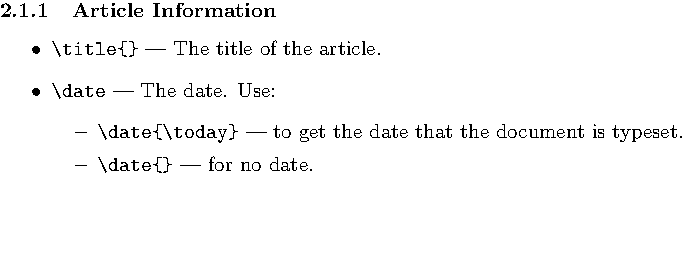
\includegraphics[width=.5\textwidth]{env3-crop}}
\end{center}

好了,请你现在照猫画虎,再来一个 subsubsection,标题叫 Author Information。模仿上面的东西,
来得到下面的东西:

\begin{minted}[fontsize=\small,baselinestretch=1,
  linenos=true,numbersep=3pt,
  frame=leftline,framesep=10pt,rulecolor=\color{lightgray},
  xleftmargin=2cm,%xrightmargin=4cm,
  gobble=2
  ]{latex}
  \subsubsection{Author Information}
  \label{sec:author-information}
  
  The basic article class only provides the one command:
  \begin{itemize}
  \item \verb|\author{}| --- The author of the document.
  \end{itemize}
  
  It is common to not only include the author name, but
  to insert new lines (\verb|\\|) after and add things
  such as address and email details.  For a slightly more
  logical approach, use the AMS article class (\emph{amsart})
  and you have the following extra commands:
  
  \begin{itemize}
  \item \texttt{address} --- The author's address.  Use the
    new line command (\verb|\\|) for line breaks.
  \item \texttt{thanks} --- Where you put any acknowledgments.
  \item \texttt{email} --- The author's email address.
  \item \texttt{urladdr} --- The URL for the author's web page.
  \end{itemize}
\end{minted}

显示效果:
\begin{center}
  \fbox{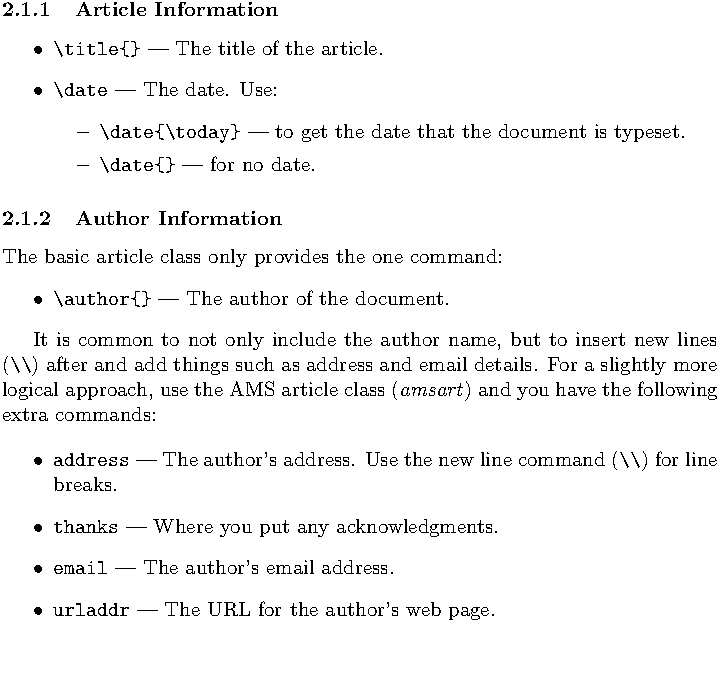
\includegraphics[width=.6\textwidth]{env4}}
\end{center}

怎么样,不太困难吧? 目前为止,我们用到的无非是表[~\ref{tab:keys}]中列出的这几个快捷键操作
而已:

\begin{table}[!htbp]
  \centering
  \caption{常用快捷键}\label{tab:keys}
  \begin{tabu*}to .5\textwidth {X[r]|X[l]}
    \hline
    \rowfont[c]{\bfseries}快捷键&功用\\\hline
    \Cj{}&换行带缩进\\
     \Cc\Cm{}&输入Macro\\
     \Cc\Cs{}&新起一个章节\\
     \Cc\Ce{}&新起一个环境\\
     \MEnter{}&换行带 \textbackslash\texttt{item}\\\hline
  \end{tabu*}
\end{table}

好,趁热打铁,再起一个小节,
\begin{enumerate}
\item \Cc\Cs{} subsection \Cj
\item Sectioning Commands \Cj\Cj
\end{enumerate}
再添加一些文字,得到:

\begin{minted}[fontsize=\small,baselinestretch=1,
  linenos=true,numbersep=3pt,
  frame=leftline,framesep=10pt,rulecolor=\color{lightgray},
  xleftmargin=2cm,%xrightmargin=4cm,
  gobble=2
  ]{latex}
  % 此处略去数十行
 
  \subsection{Sectioning Commands}
  \label{sec:sectioning-commands}
  
  The commands for inserting sections are fairly intuitive.
  Of course, certain commands are appropriate to different
  document classes. For example, a book has chapters but a
  article doesn't.
  
  % A simple table. The center environment is first set up,
  % otherwise the table is left aligned.  The tabular environment
  % is what tells Latex that the data within is data for the table.
\end{minted}

% 再看看效果:
% \begin{center}
%   \fbox{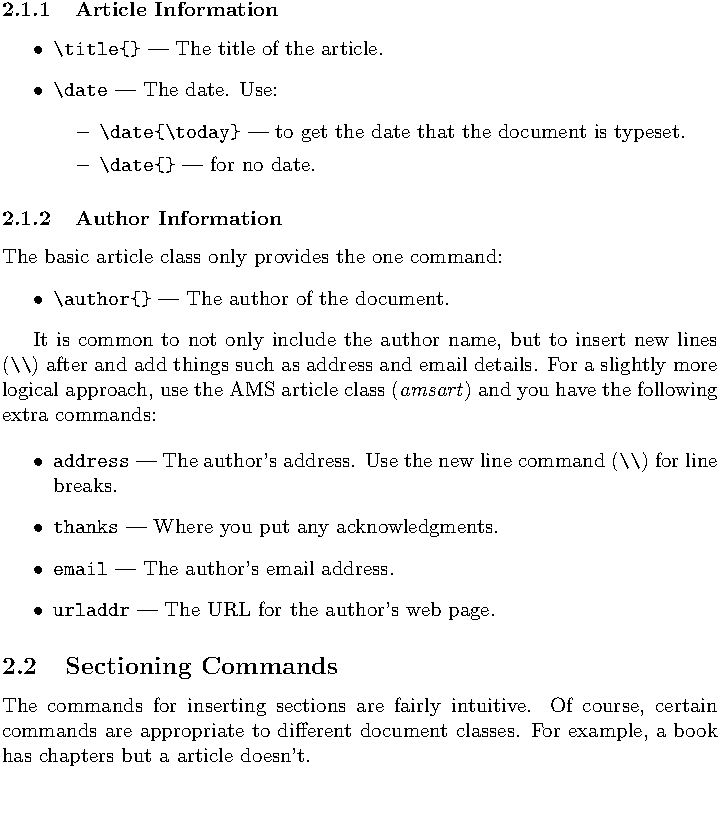
\includegraphics[width=.5\textwidth]{env5}}
% \end{center}
没什么新鲜东西,就不看效果了。下面抓紧说说怎么画表格。

\subsection{制作表格}

在这一小节,我们来尝试一下表格的输入。先起一个新“环境”,center,自然是“居中”的意思 :
\begin{enumerate}
\item[] \Cc\Ce center \Cj
\end{enumerate}
得到:

\begin{minted}[fontsize=\small,baselinestretch=1,
  linenos=true,numbersep=3pt,
  frame=leftline,framesep=10pt,rulecolor=\color{lightgray},
  xleftmargin=2cm,%xrightmargin=4cm,
  gobble=2
  ]{latex}
  % 此处略去数十行
 
  \subsection{Sectioning Commands}
  \label{sec:sectioning-commands}
  
  The commands for inserting sections are fairly intuitive.
  Of course, certain commands are appropriate to different
  document classes. For example, a book has chapters but a
  article doesn't.
  
  % A simple table. The center environment is first set up,
  % otherwise the table is left aligned.  The tabular environment
  % is what tells Latex that the data within is data for the table.

  \begin{center}
    
  \end{center}
\end{minted}

在center环境里面,我们添加一个 tabular(表格)环境:
\begin{enumerate}
\item[] \Cc\Ce{} tabular \Cj
\end{enumerate}
这时你会看到这样的提示:
\begin{enumerate}
\item[] \texttt{(Optional) Position:}
\end{enumerate}
Optional是可有可无的意思,也就是说,你如果在意表格的位置(Position),那么就提供位置信息;
如果不在意,那么就不用管它。现在我们连「位置」意味着什么都不清楚,自然就不必管它了。直接 \Cj{},又看到提示了:
\begin{enumerate}
\item[] \texttt{Format:}
\end{enumerate}
这是问你,表格的格式,比如该有几列?每列之间要不要有竖线分割?等等。我的答案是这样:
\begin{enumerate}
\item[] \texttt{|l|l|}
\end{enumerate}
也就是:竖线(|),小写L(l),竖线(|),小写L(l),竖线(|)。小写L代表 left,也就是“左对齐”的
意思。那么,你应该恍然大悟了,不就是……竖线-左对齐-竖线-左对齐-竖线嘛。那么,举一反三,除了
小写L,我们还会见到r(右对齐)和c(居中)。现在 \Cj{},得到如下结果:

\begin{minted}[fontsize=\small,baselinestretch=1,
  linenos=true,numbersep=3pt,
  frame=leftline,framesep=10pt,rulecolor=\color{lightgray},
  xleftmargin=2cm,%xrightmargin=4cm,
  gobble=2
  ]{latex}
  % 此处略去数十行
 
  \subsection{Sectioning Commands}
  \label{sec:sectioning-commands}
  
  The commands for inserting sections are fairly intuitive.
  Of course, certain commands are appropriate to different
  document classes. For example, a book has chapters but a
  article doesn't.
  
  % A simple table. The center environment is first set up,
  % otherwise the table is left aligned.  The tabular environment
  % is what tells Latex that the data within is data for the table.

  \begin{center}
    \begin{tabular}{|l|l|}
      &
    \end{tabular}
  \end{center}
\end{minted}

现在我们开始画表格,先画一条横线:
\begin{enumerate}
\item[] \verb'\hline' \Cj
\end{enumerate}
所谓 \verb'\hline' ,顾名思义,就是 horizontal line。画完横线,开始第一行,
\begin{enumerate}
\item[] \verb'Command & Level \\ \hline' \Cj
\end{enumerate}
那个 \verb'&' 就是两列之间的分隔符,``\verb'\\'''我们见过,表示强制换行。照猫画虎,把所有的
行都加上,得到如下结果:

\begin{minted}[fontsize=\small,baselinestretch=1,
  linenos=true,numbersep=3pt,
  frame=leftline,framesep=10pt,rulecolor=\color{lightgray},
  xleftmargin=2cm,%xrightmargin=4cm,
  gobble=2
  ]{latex}
  % 此处略去数十行
 
  \subsection{Sectioning Commands}
  \label{sec:sectioning-commands}
  
  The commands for inserting sections are fairly intuitive.
  Of course, certain commands are appropriate to different
  document classes. For example, a book has chapters but a
  article doesn't.
  
  % A simple table. The center environment is first set up,
  % otherwise the table is left aligned.  The tabular environment
  % is what tells Latex that the data within is data for the table.

  \begin{center}
    \begin{tabular}{|l|l|}
      \hline 
      Command & Level \\ \hline
      \verb|\part{}| & -1 \\
      \verb|\chapter{}| & 0 \\
      \verb|\section{}| & 1 \\
      \verb|\subsection{}| & 2 \\
      \verb|\subsubsection{}| & 3 \\
      \verb|\paragraph{}| & 4 \\
      \verb|\subparagraph{}| & 5 \\
      \hline
    \end{tabular}
  \end{center}
\end{minted}

这张表格的效果应该就是下面这样:

\begin{singlespace}
\begin{center}
  \begin{tabular}{|l|l|}
    \hline 
    Command & Level \\ \hline
    \verb|\part{}| & -1 \\
    \verb|\chapter{}| & 0 \\
    \verb|\section{}| & 1 \\
    \verb|\subsection{}| & 2 \\
    \verb|\subsubsection{}| & 3 \\
    \verb|\paragraph{}| & 4 \\
    \verb|\subparagraph{}| & 5 \\
    \hline
  \end{tabular}
\end{center}
\end{singlespace}

好了,表格画完了。再添加点文字:

\begin{minted}[fontsize=\small,baselinestretch=1,
  linenos=true,numbersep=3pt,
  frame=leftline,framesep=10pt,rulecolor=\color{lightgray},
  xleftmargin=2cm,%xrightmargin=4cm,
  gobble=2
  ]{latex}
  % 此处略去数十行
 
  \begin{center}
    \begin{tabular}{|l|l|}
      \hline 
      Command & Level \\ \hline
      \verb|\part{}| & -1 \\
      \verb|\chapter{}| & 0 \\
      \verb|\section{}| & 1 \\
      \verb|\subsection{}| & 2 \\
      \verb|\subsubsection{}| & 3 \\
      \verb|\paragraph{}| & 4 \\
      \verb|\subparagraph{}| & 5 \\
      \hline
    \end{tabular}
  \end{center}

  Numbering of the sections is performed automatically
  by \LaTeX{}, so don't bother adding them explicitly,
  just insert the heading you want between the curly braces.
  If you don't want sections number, then add an asterisk (*)
  after the section command, but before the first curly
  brace, e.g., \verb|section*{A Title Without Numbers}|.
\end{minted}

现在编译一下,看看效果:
\begin{center}
  \fbox{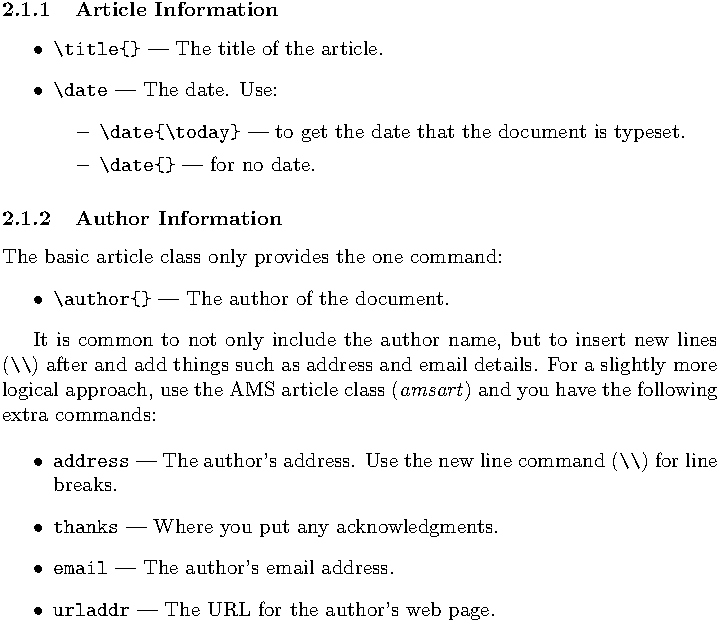
\includegraphics[width=.9\textwidth]{env6-crop-1}}
\end{center}
\begin{center}
  \fbox{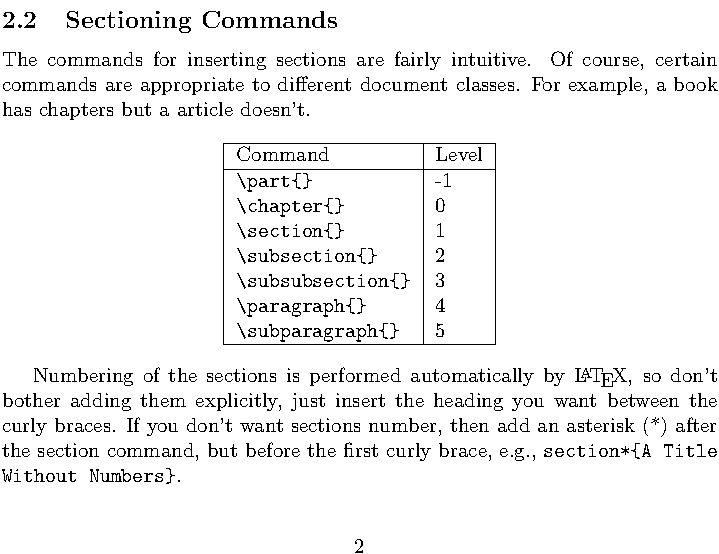
\includegraphics[width=.9\textwidth]{env6-crop-2}}
\end{center}


\subsection{引用参考文献}

现在我们讲讲“参考文献”。其实还是个environment,叫thebibliography。试试吧,
\begin{enumerate}
\item[] \Cc\Ce{} thebibliography \Cj
\end{enumerate}
mini buffer 提示:
\begin{enumerate}
\item[] \texttt{Label for BibItem: 99}
\end{enumerate}
这是问你,在引用参考文献时,采用两个字符宽的标签是否合适?你知道, 参考文献在文章中被引用到
的时候,不都是以 [1],[2]...[99] 这样的形式出现吗?所谓“两个字符的宽度”,也就是说方括号里的
数字不超过两个,也就是说你的文章中最多可以有 [1]...[99] 99个文献索引。这对于一篇普通的文章
来说肯定是足够多了。

按\Cj{},mini buffer 提示:
\begin{enumerate}
\item[] \texttt{(Optional) Bibitem label:}
\end{enumerate}
这是问你,要不要给每个参考文献条目加个标签?不理它, 按\Cj{}, mini buffer 提示:
\begin{enumerate}
\item[] \texttt{Add key (default none):}
\end{enumerate}
这是必须要理的。所谓 key ,实际上就是一条参考文献的“标识号”,它是和前面我们见到
的 \verb'\cite{}' 命令配合使用的。在引用一条参考文献时,就必然要通过它的标识号来唯一地找到
它。比如 \verb'\cite{lamport94}' 就是要从参考文献列表中找到 \texttt{lamport94}所对应的那一条。
没明白?那么我们先给它一个 key ,等会儿编译一下,看看效果就明白了。输入:\texttt{lamport94}
\Cj{},得到如下效果:

\begin{minted}[fontsize=\small,baselinestretch=1,
  linenos=true,numbersep=3pt,
  frame=leftline,framesep=10pt,rulecolor=\color{lightgray},
  xleftmargin=2cm,%xrightmargin=4cm,
  gobble=2
  ]{latex}
  \begin{thebibliography}{99}
  \bibitem{lamport94}
  \end{thebibliography}
\end{minted}

现在只需要把参考文献写进去就行了:

\begin{minted}[fontsize=\small,baselinestretch=1,
  linenos=true,numbersep=3pt,
  frame=leftline,framesep=10pt,rulecolor=\color{lightgray},
  xleftmargin=2cm,%xrightmargin=4cm,
  gobble=2
  ]{latex}
  \begin{thebibliography}{99}
  \bibitem{lamport94}
    Leslie Lamport,
    \emph{\LaTeX: A Document Preparation System}.
    Addison Wesley, Massachusetts,
    2nd Edition,
    1994.
  \end{thebibliography}
\end{minted}

再加一条:
\begin{enumerate}
\item \MEnter{} \Cj{} simple \Cj
\item \texttt{Andrew Roberts,} \Cj
\item \verb'\emph{A simple article to illustrate document structure}.' \Cj
\item \texttt{Wikibooks,}
\item \texttt{2003.}
\end{enumerate}
于是得到:

\begin{minted}[fontsize=\small,baselinestretch=1,
  linenos=true,numbersep=3pt,
  frame=leftline,framesep=10pt,rulecolor=\color{lightgray},
  xleftmargin=2cm,%xrightmargin=4cm,
  gobble=2
  ]{latex}
  \begin{thebibliography}{99}
  \bibitem{lamport94}
    Leslie Lamport,
    \emph{\LaTeX: A Document Preparation System}.
    Addison Wesley, Massachusetts,
    2nd Edition,
    1994.
  \bibitem{simple}
    Andrew Roberts,
    \emph{A simple article to illustrate document structure}.
    Wikibooks,
    2003.
  \end{thebibliography}
\end{minted}

编译一下,看看结果吧。还记得前面我们遇到过的 \verb'\cite{}'命令吗?回去看看,加上参考文献之
后它的样子,其实很简单,就是个``\texttt{[1]}'',在第1节的第2行。
一篇像模像样的科技论文到此就算是大功告成了。\texttt{simple.tex}的完整文件可以通过下面这个链
接找到:
\begin{itemize}
\item \url{https://en.wikibooks.org/wiki/LaTeX/simple.tex}
\end{itemize}

\section{小结}
本章我们利用Andrew Roberts的\texttt{simple.tex}了解了一下\LaTeX{}中最常用的命令和环境,同时
也熟悉了一下Emacs的基本键盘操作,在此做个小结。

\LaTeX{}最常用到的命令和环境:
\begin{center}
  \begin{tabu*}{|l|l|l|}
    \hline \verb'\title{}'&\verb'\author{}'&\verb'\date{}'\\\hline
    \verb'\section{}'&\verb'\subsection{}'&\verb'\subsubsection'\\\hline
    \texttt{itemize}&\texttt{center}&\texttt{tabular}\\\hline
  \end{tabu*}
\end{center}

最基本的Emacs快捷键:\label{p:keys}%(大多以\Cx{}开头)
\vskip 1ex
\begin{onehalfspace}
  \begin{itemize}
  \item[] \textbf{文件操作:}
    \begin{tabu}{rl}\hline
      打开文件:&\Cx\Cf{}\\
      存盘:&\Cx\Cs{}\\
      关掉文件:&\Cx\LKey{k}\\
    \end{tabu}
  \item[] \textbf{编辑操作:}
    \begin{tabular}{rlrl}\hline
      终止命令:&\Cg{}&设置标记:&\Ctrl{}\LKeySpace{}\\
      换行缩进:&\Cj{}&缩进:&\Ci{}\\
      取消操作:&\Cslash{}&删除字符:&\Cd{}\\
      剪切:&\Ck{}&粘贴:&\Cy{}\\\hline
    \end{tabular}
  \item[] \textbf{移动光标:}
    \begin{tabular}{rlrl}
      向前:&\Cf{}&向后:&\Cb{}\\
      行首:&\Ca{}&行尾:&\Ce{}\\
      下一行:&\Cn{}&\hspace{1em}上一行:&\Cp{}\\
      \hspace{1em}下一页:&\Cv{}&上一页:&\Mv{}\\
    \end{tabular}
  \item[] \textbf{窗口操作:}
    \begin{tabular}{rlrl}\hline
      横分:&\Cx\LKey{2}&纵分:&\Cx\LKey{3}\\
      \hspace{1em}保留我:&\Cx\LKey{1}&关掉我:&\Cx\LKey{0}\\
      切换:&\Cx\LKey{o}&&\\\hline
    \end{tabular}
  \item[] \textbf{寻求帮助:}
    \begin{tabular}{rlrl}
      教程:&\Ch\LKey{t}&info:&\Ch\LKey{i}\\
      \hspace{1em}快捷键:&\Ch\LKey{k}&\hspace{1em}函数:&\Ch\LKey{f}\\
      变量:&\Ch\LKey{v}&&\\\hline
    \end{tabular}
  \end{itemize}
\end{onehalfspace}
\vskip 2ex
最基本的AUC\TeX{}快捷键(大多以\Cc{}开头)

\begin{onehalfspace}
  \begin{center}
    \begin{tabu}{rl|rl}\hline
      环境:&\Cc\Ce{}&章节:&\Cc\Cs{}\\
      命令:&\Cc\Cm{}&换行:&\MEnter{}\\
      编译:&\Cc\Cc{}&查看:&\Cc\Cv\\\hline
    \end{tabu}
  \end{center}
\end{onehalfspace}

有了这些入门基础,我们已经可以应付要求不甚严格的文章排版了。但如果想排版出高质量的毕业论
文,hmm...,同志仍需努力。

在后续章节里,我们将简要介绍如下一些内容:
\begin{enumerate}
\item 如何插入图片
\item 如何写数学公式
\item 如何插入程序代码
\item 如何写中文
\item 如何使用毕业论文模版
% \item 如何做幻灯片
% \item Emacs org-mode
\end{enumerate}

\chapter{入门以后}

站在上一章的入门基础之上,本章我将介绍一些更为有趣的东西。这些貌似“高级”的技术其实也不复杂,
无非是再多认识几个命令和环境罢了。

\section{插入图片}

\begin{minted}[fontsize=\small,baselinestretch=1,
  linenos=true,numbersep=3pt,
  frame=leftline,framesep=10pt,rulecolor=\color{lightgray},
  xleftmargin=2cm,%xrightmargin=4cm,
  gobble=2
  ]{latex}
  \documentclass{article}
  
  \usepackage{graphicx}
  \graphicspath{{./figs/}{./}}
  
  \begin{document}
  
\includegraphics[width=5cm]{tux}
  \end{document}
\end{minted}

怎么样,能看明白吗?插入图片用到了三个新命令:
\begin{enumerate}
\item \verb'\usepackage{graphicx}', 这是在说「我要用到一个名字叫 graphicx 的package(宏
  包)」。这很类似于我们C编程时常用的 \verb'#include<stdio.h>'。\verb'\includegraphics{}'就
  是这个宏包提供的命令之一。想详细了解 graphicx的话,你可以打开一个命令终端,敲命
  令:\texttt{texdoc graphicx}。\texttt{texdoc}是TeXLive提供的专门用来看各种宏包手册的小工
  具。你可以通过\texttt{texdoc -h}命令来粗略了解它的用法。
\item \verb'\graphicspath{{./figs/}{./}}', 显然这是在指明graphics(图片)所在的path(路径,位
  置),也就是说,当你编译的时候,\LaTeX{}会到你指定的地方去找要插入的图片。在这里,我指定
  了两个地方:
  \begin{enumerate}
  \item \texttt{./figs/},当前目录下的\texttt{figs}目录。如果在这里没有找到,那么就去下面的
    目录里接着找;
  \item \texttt{./},也就是当前目录。如果在这个目录里还是没找到想插入的图片,那么编译器就要
    报错了。
  \end{enumerate}
\item \verb'
\includegraphics[width=5cm]{tux}',这显然就是在插入图片了。
  \begin{enumerate}
  \item 图片的名字叫 \texttt{tux.pdf}, 后缀(\texttt{.pdf})可以被省略掉。显
    然 \texttt{tux.pdf} 应该被存放在 \texttt{./} 或者 \texttt{./figs/} 中,才能被找到。我喜
    欢PDF图片,因为它可以自由缩放。你当然可以插入jpeg、png图片。
  \item 宽度是5cm,也可以是相对宽度,比如 \verb'[width=.5\textwidth]' 就表示宽度等于0.5倍的行宽。
  \end{enumerate}
\end{enumerate}
如果你希望图片“居中”摆放,那自然是要用到 center 了:

\begin{minted}[fontsize=\small,baselinestretch=1,
  linenos=true,numbersep=3pt,
  frame=leftline,framesep=10pt,rulecolor=\color{lightgray},
  xleftmargin=2cm,%xrightmargin=4cm,
  gobble=2
  ]{latex}
  \documentclass{article}
  
  \usepackage{graphicx}
  \graphicspath{{./figs/}{./}}
  
  \begin{document}
  \begin{center}
    
\includegraphics[width=5cm]{tux}
  \end{center}
  \end{document}
\end{minted}

编译后的效果大致就是这样,居中,5cm宽。
\begin{center}
  
\includegraphics[width=5cm]{tux}
\end{center}

\subsection{Figure环境}
\label{sec:figure}

“哎,似乎应该加上图片说明吧?比如,【图1: Linux图标】?” 这个容易,只要用到一个新的
environment,叫figure。

\Cc\Ce figure \Cj{},mini buffer提示:
\begin{enumerate}
\item[] \texttt{(Optional) Float position:}
\end{enumerate}
这是在问你图片放在那里比较好啊?是靠上?还是靠下?还是懒得操心?如果没概念,那还是让LaTeX
来决定吧,\Cj{}, mini buffer 提示:
\begin{enumerate}
\item[] \texttt{Caption:}
\end{enumerate}
这是在提示你输入图片的说明文字。那么输入:
\begin{enumerate}
\item[] \texttt{Linux logo}
\end{enumerate}
mini buffer 提示:
\begin{enumerate}
\item[] \texttt{Center? (y or n):} 
\end{enumerate}
当然选:
\begin{enumerate}
\item[] \texttt{y}
\end{enumerate}
mini buffer 提示:
\begin{enumerate}
\item[] \texttt{Label: fig:}
\end{enumerate}
这是要你给图片打个标签,以后方便索引到它。那么就给个标签:
\begin{enumerate}
\item[] \texttt{linux-logo}
\end{enumerate}
于是得到:

\begin{minted}[fontsize=\small,baselinestretch=1,
  linenos=true,numbersep=3pt,
  frame=leftline,framesep=10pt,rulecolor=\color{lightgray},
  xleftmargin=2cm,%xrightmargin=4cm,
  gobble=2
  ]{latex}
  \documentclass{article}
  
  \usepackage{graphicx}
  \graphicspath{{./figs/}{./}}
  
  \begin{document}
  \begin{figure}
    \centering
    
    \caption{Linux logo}
    \label{fig:linux-logo}
  \end{figure}
  \end{document}
\end{minted}

现在你建立了一个完美的图片环境,别忘了把图片放进去。当然放在第9行:

\begin{minted}[fontsize=\small,baselinestretch=1,
  linenos=true,numbersep=3pt,
  frame=leftline,framesep=10pt,rulecolor=\color{lightgray},
  xleftmargin=2cm,%xrightmargin=4cm,
  gobble=2
  ]{latex}
  \documentclass{article}
  
  \usepackage{graphicx}
  \graphicspath{{./figs/}{./}}
  
  \begin{document}
  \begin{figure}
    \centering
    
\includegraphics[width=5cm]{tux}
    \caption{Linux logo}
    \label{fig:linux-logo}
  \end{figure}
  \end{document}
\end{minted}

编译后的效果如图\ref{fig:linux-logo}所示。

\subsection{\textbackslash{}\texttt{label\{\}}和 \textbackslash{}\texttt{ref\{\}}的用法}
\label{sec:label}

\verb'\label{}'到底怎么用?来看下面的例子就明白了。

\begin{minted}[fontsize=\small,baselinestretch=1,
  linenos=true,numbersep=3pt,
  frame=leftline,framesep=10pt,rulecolor=\color{lightgray},
  xleftmargin=2cm,%xrightmargin=4cm,
  gobble=2
  ]{latex}
  \documentclass{article}
  
  \usepackage{graphicx}
  \graphicspath{{./figs/}{./}}
  
  \begin{document}
  \begin{figure}
    \centering
    
\includegraphics[width=5cm]{tux}
    \caption{Linux logo}
    \label{fig:linux-logo}
  \end{figure}

  Figure~\ref{fig:linux-logo} is the famous Linux Tux!
  图\ref{fig:linux-logo}所示就是大名鼎鼎的Linux吉祥物!
  \end{document}
\end{minted}

编译一下,看看效果吧。

\begin{figure}
  \centering
  
\includegraphics[width=5cm]{tux}
  \caption{Linux logo}
  \label{fig:linux-logo}
\end{figure}

Figure~\ref{fig:linux-logo} is the famous Linux Tux!
图\ref{fig:linux-logo}所示就是大名鼎鼎的Linux吉祥物!

\verb'\label{}' 和 \verb'\ref{}' 总是配合使用的,一个用来打标签,另一个用来找到它。而且这
两个命令可以被用在任何你需要的地方,非常方便。比如,

\begin{minted}[fontsize=\small,baselinestretch=1,
  linenos=true,numbersep=3pt,
  frame=leftline,framesep=10pt,rulecolor=\color{lightgray},
  xleftmargin=2cm,%xrightmargin=4cm,
  gobble=2
  ]{latex}

  % 本文的第一章标题
  \chapter{工欲善其事,必先利其器}
  \label{cha:pre-requisite}   % 章标签

  % 本文中的某张表格
  \begin{table}[!htbp]
    \centering
    \caption{常用快捷键}\label{tab:keys}  % 表格标签
    \begin{tabu*}to .5\textwidth {X[r]|X[l]}
      \hline
      \rowfont[c]{\bfseries}快捷键&功用\\\hline
      \Cj{}&换行带缩进\\
      \Cc\Cm{}&输入Macro\\
      \Cc\Cs{}&新起一个章节\\
      \Cc\Ce{}&新起一个环境\\
      \MEnter{}&换行带{\verb|\item|}\\\hline
    \end{tabu*}
  \end{table}

  % 在文中某处有这样一行
  最基本的Emacs快捷键(大多以\Cx{}开头)\label{p:keys} % 任意标签

  %%% 下面让我们来使用(索引)上面的标签
  
  \begin{enumerate}
  \item 本文的第~\ref{cha:pre-requisite}章介绍了一个简单、% 索引某章
    高效的工作环境;
  \item 在表~\ref{tab:keys}中列出了几个最常用的快捷键; % 索引某表
  \item 在第~\pageref{p:keys}页列出了更多的快捷键。    % 索引某页
  \end{enumerate}
\end{minted}

上述代码就可以生成如下的效果,不仅数字是正确的,而且它们都是hyperlink,用鼠标点一下试试。
\begin{enumerate}
\item 本文的第\ref{cha:pre-requisite}章介绍了一个简单、高效的工作环境;
\item 在表\ref{tab:keys}中列出了几个最常用的快捷键;
\item 在第\pageref{p:keys}页列出了更多的快捷键。
\end{enumerate}

\subsubsection*{快捷地插入标签和索引}

插入标签和索引也是有快捷键的。\Cc\biolinumKeyGlyph{parenleft}就是要插入标签,mini
buffer提示:
\begin{enumerate}
\item[] \texttt{Label: cha:}
\end{enumerate}
如果你不是要插入章标签,那么可以把\texttt{cha}改成其它你认为合适的字符。通常Emacs会根据光
标所在的环境给出不同的提示,如果光标在
\begin{itemize}
\item Figure里,它就提示\texttt{fig:};
\item Table里,它就提示\texttt{tab:};
\item 正文中其它什么地方,它就提示 \texttt{cha:}或者 \texttt{sec:}。
\end{itemize}
现在,在提示下输入一个简短而好记的标签名称,以便后面可以轻松找到它。

要插入索引(\verb'\ref{}')的话,敲 \Cc\biolinumKeyGlyph{parenright},mini buffer 提示:
\begin{itemize}
\item[] \texttt{SELECT A REFERENCE FORMAT}
\item[] \verb'[^M]  \ref'
\item[] \verb'[p]   \pageref' 
\end{itemize}
这是让你选择索引格式,如果想索引某页的话,就选\texttt{[p]}。其它任何情况,都选择
\verb'[^M]',也就是直接回车,\Enter{}。根据你的选择,Emacs会弹出新的buffer,方便你找到要引
用的标签。

\section{数学公式}
\label{sec:math}

举个简单的例子吧:

\begin{minted}[fontsize=\small,baselinestretch=1,
  linenos=true,numbersep=3pt,
  frame=leftline,framesep=10pt,rulecolor=\color{lightgray},
  xleftmargin=2cm,%xrightmargin=4cm,
  gobble=2
  ]{latex}
  \documentclass{article}
  \begin{document}
  This is a simple math example: $c^2=a^2+b^2$
  \end{document}
\end{minted}

结果是这样:
\begin{itemize}
\item[] This is a simple math example: $c^2=a^2+b^2$
\end{itemize}

美元符号(\verb'$')在 \LaTeX{}里面是特殊字符。夹在两个美元符号之间的东西,会被当做数学公式来排版。
如果想让数学公式独占一行的话,就用双美元符号(\verb'$$'),比如,
$$(1+x)^n=\sum_{k=0}^n\binom{n}{k}x^k$$
就是\verb'$$(1+x)^n=\sum_{k=0}^n\binom{n}{k}x^k$$'的输出结果。还不难看懂吧?
\begin{itemize}
\item \verb'\sum' $\Rightarrow\sum$
\item \verb'\binom{n}{k}' $\Rightarrow\binom{n}{k}$
\item 下划线(\texttt{\_})后面跟下标,如果下标不止一个字符,那么就要用花括号
  (\texttt{\{\}})括起来。比如,\verb'A_1 + A_{100}' $\Rightarrow{}A_1 + A_{100}$;
\item 上箭头(\verb'^')后面跟上标,用法和下划线一样。比如,\verb'2^2 \times 2^{32}'
  $\Rightarrow$ $2^2\times{}2^{32}$。 
\end{itemize}

那么,去哪里找这些数学符号呢?很简单,Google一下“latex math”,就什么都有了。“天啊,谁能记住
那么多数学符号啊?!”。\LaTeX{}的数学排版功能博大精深,各式各样的数学符号、怪异字符无所不及,
当然用不着都记住。你只要记住上面我们提到的几条,应该就足以应付毕业论文了。如果你要经常对付
复杂数学公式的话,那么最好把《The \LaTeX{} Companion》\cite{Goossens94a}这本书的第八章
(Higher Mathematics)打印下来放在手边,随用随查就好了。Google一下“latex math chapter 8”。

\section{插入程序代码}
\label{sec:code}

还是从一个小例子开始吧。

\rule{0.9\textwidth}{.4pt}

\begin{minipage}[t]{.45\linewidth}
  代码:
  \begin{center}
    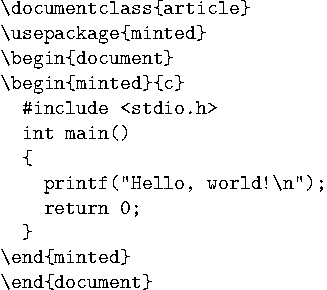
\includegraphics[width=\textwidth]{code}
  \end{center}
\end{minipage}
\hfill\vline\hfill
\begin{minipage}[t]{.45\linewidth}
  效果:
  \vspace{4.6em}
  \begin{minted}[baselinestretch=1,xleftmargin=-2em]{c}
    #include <stdio.h>
    int main()
    {
      printf ("Hello, world!\n");
      return 0;
    }
  \end{minted}
\end{minipage}
\begin{center}
\rule{0.9\textwidth}{.1pt}
\end{center}

首先要\verb'\usepackage{minted}'。minted是用于美化代码排版的\LaTeX{}宏包,有了它,你可以把
几乎所有编程语言的代码排版得像你们老师那样道貌岸然,而且是彩色的。不过,对于毕业论文来说,
还是采用黑白排版比较好。彩色排版如果黑白打印,效果就很模糊了。当然你可以选择彩色打印,但那
很费钱啊。

想详细了解minted的用法,就:\texttt{texdoc minted}。minted宏包提供了一个新环境,就
叫minted ,把你的程序放在 \verb'\begin{minted}'和 \verb'\end{minted}'之间就行
了。\verb'\begin{minted}'后面的 \verb'{c}'当然是说,插入的程序是用C语言写的。
  
怎么?程序太长,拷贝进来太麻烦?那么可以这样:
    
\begin{minted}[fontsize=\small,baselinestretch=1,
  linenos=true,numbersep=3pt,
  frame=leftline,framesep=10pt,rulecolor=\color{lightgray},
  xleftmargin=2cm,%xrightmargin=4cm,
  gobble=2
  ]{latex}
  \documentclass{article}
  \usepackage{minted}
  \begin{document}
  
  \inputminted{c}{hello.c}
  
  \end{document}
\end{minted}

简单吧?\texttt{hello.c} 当然要和你的 \TeX{} 文件在同一个目录下,否则你要指明详细路径。

minted宏包提供了丰富的命令,可以支持数十种编程语言,后台调用强大的pygments来打扮你的程序
代码,可以把程序以各种你能想到的方式排版出来。当然,使用 minted 的前提条件是,系统里已经安
装好了python和pygments。这一点在minted的手册里已经说得很清楚了。关于强大的pygments,
你该去它的网站看看:\url{http://pygments.org/}。

\section{处理中文}
\label{sec:cn}

如果你的Emacs配置和我的一样,那么输入中文就是“piece of cake”,当然你得安装了中文输入法,我
用的是fcitx\footnote{\url{https://fcitx-im.org/wiki/Fcitx}},还不错,挺好用的。

现在,打开一个全新的\texttt{tex}文件,比如\texttt{hello.tex},在里面写\texttt{article},然
后敲\Tab{}(TAB)键,一个现成的\LaTeX{}文件模板立时会展现在你的面前。这个模版里有你写一篇漂
亮中文文章所需要的一切。光标就停在 \verb'\title{}' 的花括号里,那么就开始用中文填空
吧。Happy \TeX{}ing!

附录[\ref{app:article}]中列出了这一\texttt{article}模板的全部内容。在这里我们简单解释一下其中
和中文相关的几行。

\begin{minted}[fontsize=\small,baselinestretch=1,
  linenos=true,numbersep=3pt,firstnumber=17,
  frame=leftline,framesep=10pt,rulecolor=\color{lightgray},
  xleftmargin=2cm,%xrightmargin=4cm,
  gobble=2
  ]{latex}
  \usepackage{xltxtra} %fontspec,xunicode are loaded here.
  \defaultfontfeatures{Mapping=tex-text}
  \setsansfont{DejaVu Sans}
  \setmainfont{DejaVu Serif}
\end{minted}

\begin{enumerate}\setcounter{enumi}{16}
\item \verb'\usepackage{xltxtra}'。我们用的\LaTeX{} Engine,或者说我们用来编
  译 \texttt{tex}文件的程序,
  是\XeLaTeX{}\footnote{\url{https://en.wikipedia.org/wiki/XeTeX}}。它的正常编译依赖
  于 \texttt{xltxtra, fontspec, xunicode}这几个宏包。所以我们
  要 \verb'\usepackage{xltxtra}',加载\texttt{xltxtra}的同时,其它两个宏包会被自动加载,所
  以就不必写上来了。
\item \verb'\defaultfontfeatures{Mapping=tex-text}',这是\texttt{fontspec}的一个选项,作用
  就是让\texttt{---}变成---,也就是让三根短横线组成一个破折号。
\item \verb'\setsansfont{DejaVu Sans}'和 \verb'\setmainfont{DejaVu Serif}'是设置英文字体。
\end{enumerate}

如果只是写英文文章的话,有上面这几行就够了。如果要写中文,那么就要加上下面这些:

\begin{minted}[fontsize=\small,baselinestretch=1,
  linenos=true,numbersep=3pt,firstnumber=21,
  frame=leftline,framesep=10pt,rulecolor=\color{lightgray},
  xleftmargin=2cm,%xrightmargin=4cm,
  gobble=2
  ]{latex}
  \usepackage{xeCJK}
  \xeCJKDeclarePunctStyle{ mine }
  {
    min-bound-to-kerning    = true,
    kerning-margin-minimum  = .2em,
  }
  \xeCJKsetup{PunctStyle=mine}
  \xeCJKsetwidth{“”《》、()}{1.2ex}
  \xeCJKsetkern{:}{(}{1ex}
  \xeCJKsetkern{;}{(}{1ex}
  \setCJKmainfont[BoldFont={Adobe Heiti Std}]{Adobe Song Std}
  \setCJKsansfont{Noto Sans CJK SC Regular}
  \setCJKmonofont{Noto Sans Mono CJK SC Regular}
  \setCJKfamilyfont{hei}{Adobe Heiti Std}
  \setCJKfamilyfont{song}{Adobe Song Std}
  \setCJKfamilyfont{kai}{Adobe Kaiti Std} % e.g. \CJKfamily{kai}
  \newCJKfontfamily\quotefont{Adobe Kaiti Std}
  
  \newcommand{\ziju}[1]{\renewcommand{\CJKglue}{\hskip #1}}
\end{minted}

\begin{enumerate}\setcounter{enumi}{20}
\item \verb'\usepackage{xeCJK}'。xeCJK是一个\XeLaTeX{}宏包,用于排版中日韩(CJK)文字。
  \cite{xecjk} 想了解更多,就\texttt{texdoc xecjk},很值得一读;
\item[22-30] 这几行都是用来调整中文标点排版的,可有可无。相邻的两个中文标点之间总是有遥不可
  及距离,如果你想把它们拉近,不妨照猫画虎地设置一下;
\item[31-33] 这三行用来选择中文字体,非要不可。Adobe Song Std就是Adobe的标准宋体字;Adobe
  Heiti Std是黑体字。你当然也可以选用其它字体,比如WenQuanYi Zen Hei就是不错的开源字体。Noto
  Sans CJK是Google提供的开源字体;
\item[34-37] 这四行用于在文章中间变换字体,如果你没这个需求,就不必管它。
  举几个例子,
  \begin{itemize}
  \item \{\verb'\CJKfamily{kai}'楷体\} $\Rightarrow$ {\CJKfamily{kai}楷体}
  \item \{\verb'\CJKfontspec{FZGuLi-S12S}'方正古隶简体\} $\Rightarrow$
    {\CJKfontspec{FZGuLi-S12S}方正古隶简体}
  \item \{\verb'\CJKfontspec{FZXingKai-S04S}'方正行楷简体\} $\Rightarrow$
    {\CJKfontspec{FZXingKai-S04S}方正行楷简体}
  \end{itemize}
  还不错吧?但前提是你的系统里要已经装上了这些字体才行。
\item[39] 这一行用于调整字间距离。比如,
  \begin{itemize}
  \item \verb'{\ziju{1mm}一毫米字距}' $\Rightarrow$ {\ziju{1mm}一毫米字距}
  \item \verb'{\ziju{3mm}三毫米字距}' $\Rightarrow$ {\ziju{3mm}三毫米字距}
  \item \verb'{\ziju{5mm}五毫米字距}' $\Rightarrow$ {\ziju{5mm}五毫米字距}
  \item \verb'{\ziju{1cm}一厘米字距}' $\Rightarrow$ {\ziju{1cm}一厘米字距}
  \end{itemize}
  写论文的时候,应该不需要这样辛苦地手工调整字距。直接套用论文模板,一切就很完美了。
\end{enumerate}

\chapter{完美的毕业论文}
\label{cha:thesis}

写毕业论文,像结婚一样,是一生一次的大事情。潦草而失败的论文,就像失败的婚姻,总要一次次地
返工,在痛苦中煎熬,直到你遇见ta,带你摆脱迷茫、痛苦,登上幸福的彼岸\footnote{我说的当然
  是\LaTeX{}。}。

\begin{itemize}
\item[] 写普通文章要用 \verb'\documentclass{article}';
\item[] 写报告要用 \verb'\documentclass{report}';
\item[] 写书要用 \verb'\documentclass{book}';
\item[] 写信要用 \verb'\documentclass{letter}';
\item[] 那么写毕业论文自然要用毕业论文模版了:\verb'\documentclass{swfcthesis}'。
\end{itemize}

如此关系人生的大事情,当然要为它专门建立一个目录吧。目录建好了,把论文模板 \texttt{swfcthesis.cls} 文件拷贝
进去。然后就可以用它来写你的论文了。

\section{Class文件}
\label{sec:class}

Class文件\footnote{也就是后缀为\texttt{.cls}的文件,也就是我们常说的模板文件。},它决定了你
的文章样式,比如说,纸张尺寸、页边距、行距、字距、字体、标题样式等等在class文件中都做了设
置。除此之外,我们在写\texttt{tex}文件的过程中用到的命令(Macro)也都是class文件提供的。

这里有一个值得注意的概念,排版这件事情,是由排版软件根据你(在文章中提供)的命令来进行的。
只要你的命令正确,文章的格式就必然是正确的。这就是排版软件和字处理软件,比如MS-Word,的区
别所在。利用字处理软件来写文章,你不得不既操心文章的内容,也操心文章的格式。而利用排版软件,
比如\LaTeX{}来写文章,你只需要关心文章的内容,而格式的事情,排版软件会根据你的命令来替你完
成。所以,你输入的命令必须正确、合法、合情理才行。

排版软件只能听懂class文件中提供的命令\footnote{我说谎了,实际上,在\texttt{tex}文件中,你可
  以利
  用 \texttt{\textbackslash{}newcommand\{\}}和 \texttt{\textbackslash{}renewcommand\{\}}来
  定义自己的命令。但对于初学者来说,你暂时还不必操心这个,class文件所提供的命令应该足以应付
  你目前的需求了。},所以,我们当然要对这些命令有个基本的了解。附录[\ref{app:class}]中就
是\texttt{swfcthesis.cls}文件的全部内容。我们在此做个简要介绍。简而言
之,\texttt{swfcthesis.cls}提供了如下一些基本命令:

\begin{enumerate}
\item \verb'\Title{论文标题}'
\item \verb'\Author{作者}'
\item \verb'\Advisor{指导教师姓名}'
\item \verb'\AdvisorTitle{指导教师职称}'
\item \verb'\AdvisorInfo{指导教师简介}'
\item \verb'\Month{这里填月份}'
\item \verb'\Year{这里填年份}'
\item \verb'\Univ{这里填校名}'
\item \verb'\School{这里填院名}'
\item \verb'\Subject{这里填专业}'
\item \verb'\Docname{本科毕业(设计)论文}' (目前我们只关心本科毕业论文)
\item \verb'\Abstract{这里填上中文摘要}'
\item \verb'\Keywords{这里填上关键字}'
\item \verb'\Acknowledgments{在这里感谢祖国感谢党}'
\item \verb'\enTitle{这里填上英文标题}'
\item \verb'\enAuthor{这里填上你的洋名字}'
\item \verb'\enUniv{这里填上英文校名}'
\item \verb'\enSchool{这里填上英文院名}'
\item \verb'\enAbstract{这里填上英文摘要}'
\item \verb'\enKeywords{这里填上英文关键字}'
\item \verb'\makepreliminarypages{}' 用于生成封面、摘要、英文摘要……
\item \verb'\Appendix{}' : 附录部分由此开始
\item \verb'\advisorinfopage{}' : 生成【教师简介】
\item \verb'\acknowledgmentspage{}' : 生成【鸣谢】
\end{enumerate}

\section{模板的使用}

具体如何来用这些命令呢?简而言之,\Cx\Cf{},输入一个崭新的文件名,\Cj{}。现在,面对空无一字
的Emacs窗口,你有生以来最重要的一篇文章就要开篇了,你在思考什么?其实什么都不用想,直接
敲 \texttt{thesis} \Tab{}(Tab),一个论文框架就呈现在你的眼前了,你要做的就是用你前面学到的
那些\LaTeX{}命令来填空。

在本文开始的时候(第\pageref{p:yasnippet}页),我们提到过“\Tab{}大法”是\texttt{yasnippet}的
贡献。所以,你在期待\Tab{}键能带来奇迹之前,必须先确保你的系统里已经装好了
\texttt{yasnippet}。如果还没装上,那么就执行下面的命令\cite{aptitude}:

\begin{onehalfspace}
  \begin{itemize}
  \item[] \texttt{sudo aptitude update}
  \item[] \texttt{sudo aptitude upgrade}
  \item[] \texttt{sudo aptitude install yasnippet yasnippet-snippets}
  \end{itemize}
\end{onehalfspace}

装好之后,重新加载Emacs的配置文件。很简单,在Emacs窗口里,敲
\begin{itemize}
\item[] \Mx{} \texttt{load-file} \Cj{} \verb'~/.emacs' \Cj{}
\end{itemize}

跟着本教程写论文的前提条件就是,Emacs必须工作正常,如果发现问题必须及时处理,不能将就。尤其
是在入门阶段,不要指望用一个别扭的Emacs来顺畅地写出完美的论文。

附录[\ref{app:thesis}]中列出了完整的毕业论文框架,也就是你在键入\texttt{thesis} \Tab{}后应
该看到的东西。如果奇迹没有发生,那么就要操心一下你的Emacs配置了。

假设你的Emacs环境良好,按\Tab{}键之后,本来空荡荡的Emacs buffer里现在有了一个论文框架,而且
光标就停在你要填空的第一个位置,也就是 \verb'\Title{论文标题}'的花括号里。这时,你只要键入
任何文字(通常应该是你自己的论文标题),(感谢\texttt{yasnippet})花括号里的“论文标题”四字
就会被自动替换掉。写好了论文标题,还是按\Tab{}键,光标会自动跳到下一个你需要填空的位置。如
此一直\Tab{}下去,直到光标不再跳开了,那就是你该写论文第一章内容的时候了。

论文框架里有足够多的注释,再加上你在前几章学到的本领,我相信写出一个规范、漂亮的毕业论文应该是手
到擒来的事情了。

\section{生成参考文献}
\label{sec:ref}

前面我们提到过,生成参考文献要用到 \texttt{thebibliography}环境。只要将写论文所用到的书目按
规定格式罗列其间就可以了。其实这只是一种临时、凑手的解决方案。对于那些终日埋头于书山,靠写
科技论文糊口的人来说,这种方案就显得业余而低效率了。你想啊,如果某科学家在他的1000篇大作里
都要引用相同的那么几本书,那么,这几本书岂不是要在1000篇论文
的1000个\texttt{thebibliography}里出现1000遍?万一那科学家老得连copy/paste都不知道,那可要
辛辛苦苦花几天的时间才能把这几本书的名字、作者、出版商、出版年月日抄完1000遍啊。即使他
会copy/paste,1000遍之后,手指头也要抽筋了吧。

所以,我们有必要来认识一种更专业而高效的解决方案。我们一遍都不用抄,相应的书目就能变成我们参
考文献的条目。简而言之,我们准备一个专门的\texttt{bib}文件,它的格式大致是下面这样:

\inputminted[fontsize=\small,baselinestretch=1,
linenos=true,numbersep=3pt,
frame=leftline,framesep=10pt,
rulecolor=\color{lightgray},]{latex}{tutorial.bib}

能看出点意思吗?这个小文件的内容就是本教程所引用到的所有书目。在后面第\pageref{p:ref}页的
参考文献部分里,你看到的就是这个文件的内容。

\paragraph*{这个文件是怎么来的?}

当然可以手写。\texttt{bib}文件的格式清晰易懂,照猫画虎地手写并不困难。但生活可以更轻松,如
果你引用的书籍、资料不是太冷门,那么通常只要google一下「书名 bibtex」,就可以找到相应
的\texttt{bib}条目了。有时你甚至可以从网上下载到现成的bib文件,比如全
套RFC\footnote{Request for
  Comments. \url{https://en.wikipedia.org/wiki/Request_for_Comments}}的\texttt{bib}文件。

\paragraph*{怎样使用这个文件?}

很简单,三件事:
\begin{enumerate}
\item 第一件事不用做,因为在我们的论文模板文件(\texttt{swfcthesis.cls})里已经做了。在模板
  文件里有如下一行:
  \begin{enumerate}
  \item[] \verb|\RequirePackage[backend=biber,url=false,hyperref=true,|\\
    \verb|                doi=false,isbn=false]{biblatex}|
  \end{enumerate}
  也就是说,帮我们排版参考文献的是\texttt{biblatex}宏包;
\item 在\texttt{tex}文件(你的论文)的preamble部分,也就是在\verb|\begin{document}|之前,
  加上如下一行:
  \begin{itemize}
  \item[] \verb|\addbibresource{tutorial.bib}|
  \end{itemize}
  很显然,这是在告诉\texttt{biblatex}从当前目录下的\texttt{tutorial.bib}文件里去读取参考文
  献信息。
\item 这件事也不用做了,因为在论文的框架文件(\texttt{tex}文件)里已经做好了。在
  \texttt{tex}文件的\texttt{Appendix}(附录)部分,你能看到如下一行:
  \begin{itemize}
  \item[] \verb|\printbibliography[heading={bibintoc},title={参考文献}]|
  \end{itemize}
  这就是要求排版输出参考文献。
\end{enumerate}

\section{小结}

在此我们简单回顾一下,要写出漂亮的毕业论文所应具备的必要条件:
\begin{enumerate}
\item 一套高效的工作环境
  \begin{enumerate}
  \item Debian sid;
  \item \TeX{}Live;
  \item Emacs+AUC\TeX{}+Yasnippet;
  \item Truetype中文字体。
  \end{enumerate}
\item 对Emacs基础快捷键的熟练使用;
\item \LaTeX{}的基础知识;
\end{enumerate}

只要具备了以上条件,轻松地写出一份漂亮、规范的毕业论文应该不成问题了。
先到这里吧。以后如果有时间,我会继续介绍一下
\begin{enumerate}
\item 如何用\LaTeX{} Beamer做出漂亮的演示幻灯片;
\item 如何用Emacs org-mode快速生成PDF文件。
\end{enumerate}

另外,配合本教程,我制作了一个简单的小视频,\texttt{tutorial.mkv},它应该和本文放在同一个
目录下\footnote{\url{http://cs2.swfu.edu.cn/~wx672/swfcthesis/tutorial/}}。

关于本文的任何疑问和建议,欢迎反馈到\texttt{wx672ster@gmail.com}。

\begin{flushright}
  {\Huge \fontspec{Purisa}Happy \TeX{}ing!}
\end{flushright}

%%% 正文部分到此结束。下面是『参考文献』、『指导教师简介』、『鸣谢』、『附录』
\Appendix{} % 不要动这一行!
\printbibliography[heading={bibintoc},title={参考文献}]\label{p:ref} % 输出参考文献     
\advisorinfopage{}                 % 输出指导教师简介
\acknowledgmentspage{}             % 输出鸣谢

%%% 下面是附录部分。

\chapter{与排版论文相关的软件清单}\footnotetext{
  这份清单是用如下命令获得的:
  \texttt{aptitude search '\~{}i keyword' >> pkg-list}。
  其中,keyword依次是 texlive, xterm, zathura, ... 除此之外,我还额外安装了一些Debian软件
  库中没有的中文字体,包括微软中文字体。}
\label{app:pkg}

\begin{enumerate}
\item texlive-base - TeX Live: Essential programs and files
\item texlive-bibtex-extra - TeX Live: BibTeX additional styles
\item texlive-binaries - Binaries for TeX Live
\item texlive-extra-utils - TeX Live: TeX auxiliary programs
\item texlive-fonts-extra - TeX Live: Additional fonts
\item texlive-fonts-recommended - TeX Live: Recommended fonts
\item texlive-fonts-recommended-doc - TeX Live: Documentation files for texlive-fonts-recommended
\item texlive-generic-extra - TeX Live: Generic additional packages
\item texlive-generic-recommended - TeX Live: Generic recommended packages
\item texlive-lang-chinese - TeX Live: Chinese
\item texlive-lang-cjk - TeX Live: Chinese/Japanese/Korean (base)
\item texlive-lang-english - TeX Live: US and UK English
\item texlive-latex-base - TeX Live: LaTeX fundamental packages
\item texlive-latex-base-doc - TeX Live: Documentation files for texlive-latex-base
\item texlive-latex-extra - TeX Live: LaTeX additional packages
\item texlive-latex-extra-doc - TeX Live: Documentation files for texlive-latex-extra
\item texlive-latex-recommended - TeX Live: LaTeX recommended packages
\item texlive-latex-recommended-doc - TeX Live: Documentation files for texlive-latex-recommended
\item texlive-pictures - TeX Live: Graphics, pictures, diagrams
\item texlive-pictures-doc - TeX Live: Documentation files for texlive-pictures
\item texlive-xetex - TeX Live: XeTeX and packages
\item python-pygments - syntax highlighting package written in Python   
\item auctex - integrated document editing environment for TeX etc.
\item latexmk - Perl script for running LaTeX the correct number of times
\item sawfish - window manager for X11
\item sawfish-data - sawfish architecture independent data
\item sawfish-lisp-source - sawfish lisp files
\item sawfish-merlin-ugliness - More flexible functions for sawfish
\item xterm - X terminal emulator
\item zathura - document viewer with a minimalistic interface
\item zathura-pdf-poppler - PDF support for zathura
\item google-chrome-stable - The web browser from Google
\item emacs-goodies-el - Miscellaneous add-ons for Emacs
\item emacs24 - GNU Emacs editor (with GTK+ GUI support)
\item emacs24-common-non-dfsg - GNU Emacs common non-DFSG items, including the core documentation
\item emacs24-el - GNU Emacs LISP (.el) files
\item fonts-arphic-ukai - "AR PL UKai" Chinese Unicode TrueType font collection Kaiti style
\item fonts-arphic-uming - "AR PL UMing" Chinese Unicode TrueType font collection Mingti style
\item fonts-dejavu - metapackage to pull in fonts-dejavu-core and fonts-dejavu-extra
\item fonts-dejavu-core - Vera font family derivate with additional characters
\item fonts-dejavu-extra - Vera font family derivate with additional characters (extra variants)
\item fonts-linuxlibertine - Linux Libertine family of fonts
\item fonts-tlwg-purisa - Thai Purisa font (dependency package)
\item fonts-wqy-microhei - Sans-serif style CJK font derived from Droid
\item fonts-wqy-zenhei - "WenQuanYi Zen Hei" A Hei-Ti Style (sans-serif) Chinese font
\item xfonts-wqy - WenQuanYi Bitmap Song CJK font for X
\item fcitx - Flexible Input Method Framework
\item fcitx-config-gtk - graphic Fcitx configuration tool - Gtk+ 3 version
\item fcitx-frontend-all - Flexible Input Method Framework - frontends metapackage
\item fcitx-module-cloudpinyin - Flexible Input Method Framework - cloudpinyin module
\item fcitx-module-dbus - Flexible Input Method Framework - D-Bus module and IPC frontend
\item fcitx-module-x11 - Flexible Input Method Framework - X11 module and XIM frontend
\item fcitx-modules - Flexible Input Method Framework - core modules
\item fcitx-sunpinyin - fcitx wrapper for Sunpinyin IM engine
\item fcitx-ui-classic - Flexible Input Method Framework - Classic user interface
\end{enumerate}

\chapter{中文article模板} %附录一
\label{app:article}

\inputminted[fontsize=\small,baselinestretch=1,
linenos=true,numbersep=3pt,
frame=leftline,framesep=10pt,
rulecolor=\color{lightgray},]{latex}{article.tex}

\chapter{毕业论文模板} %附录二
\label{app:thesis}

\inputminted[fontsize=\small,baselinestretch=1,
linenos=true,numbersep=3pt,
frame=leftline,framesep=10pt,
rulecolor=\color{lightgray},]{latex}{thesis.tex}

\chapter{\texttt{swfcthesis.cls}文件}
\label{app:class}

\inputminted[fontsize=\small,baselinestretch=1,
linenos=true,numbersep=3pt,
frame=leftline,framesep=10pt,
rulecolor=\color{lightgray},]{latex}{swfcthesis.cls}

\end{document} % 此行后面不要有任何文字。

%%% Local Variables:
%%% mode: latex
%%% TeX-master: t
%%% End:
